\section{IoT service slicing and task offloading for smart cities} 
\label{sec:smartcity_edge}
With the growth of the IoT industries as well as 5G, various vertical IoT use case has been emerging in the cities, and these are requiring the more agile, highly efficient capabilities. In this regard, the existing centralized IoT infrastructure based on Cloud Computing could be hard to respond immediately to citizens who use the time-sensitive services. In addition, processing the entire data generated by IoT devices is a significant burden in the centre~\cite{chen2017enabling}. As a way to solve the above problems, the research including Multi-access Edge Computing (MEC) technology to increase the real-time efficiency of data management and data transfer is being considered~\cite{wang2018network}. However, radical problems still remain since IoT platforms are placed far away from the users being taken IoT services. To conclude, to support the time-sensitive IoT services to the users, IoT service slicing and task offloading are newly defined.

\subsection{Challenges of next generation network system}
At present, the entity-based networking system has been being used to provide simple voice services and mobile services that do not call for stringent requirements. However, this one-size-fits-all network system is not suitable to cope with the diverse requirements including performance and availability and cost. To accommodate the several vertical use cases, slicing a physical network infrastructure into a logical network to provide tailored network services for a distinct application scenario has been emerged~\cite{zhang2019overview}. In addition, to realize this concept, Network Function Virtualization (NFV) and Software Defined Network (SDN) as a key enabler are driving the network paradigm shift. With the moving toward the 5G, this concept is going to be the natural solution for the upcoming network era, and it is possible to support different Service Level Agreement (SLA) by turning the ossified hardware-based networking system into software-based networking structure.

Meanwhile, with the growth of IoT industries, various vertical IoT use cases have emerged, which require high bandwidth and reduced traffic delay to support real-time IoT services. In this regard, the existing solutions based on a centralized IoT platform in the cloud have difficulty satisfying such needs. Additionally, processing the massive quantity of data generated by IoT devices is a significant burden on the central IoT platform~\cite{chen2017enabling}. To solve such problems, many research activities have considered new technologies as promising solutions, including multi-access edge computing (MEC) to increase the real-time efficiency of data management and data transfer and artificial intelligence (AI) technologies~\cite{wang2018network}. Therefore, along with advantages regarding edge computing and network slicing, it is feasible to support IoT services especially for users who need services that involve real-time.

\begin{figure}[tb!]
\centering
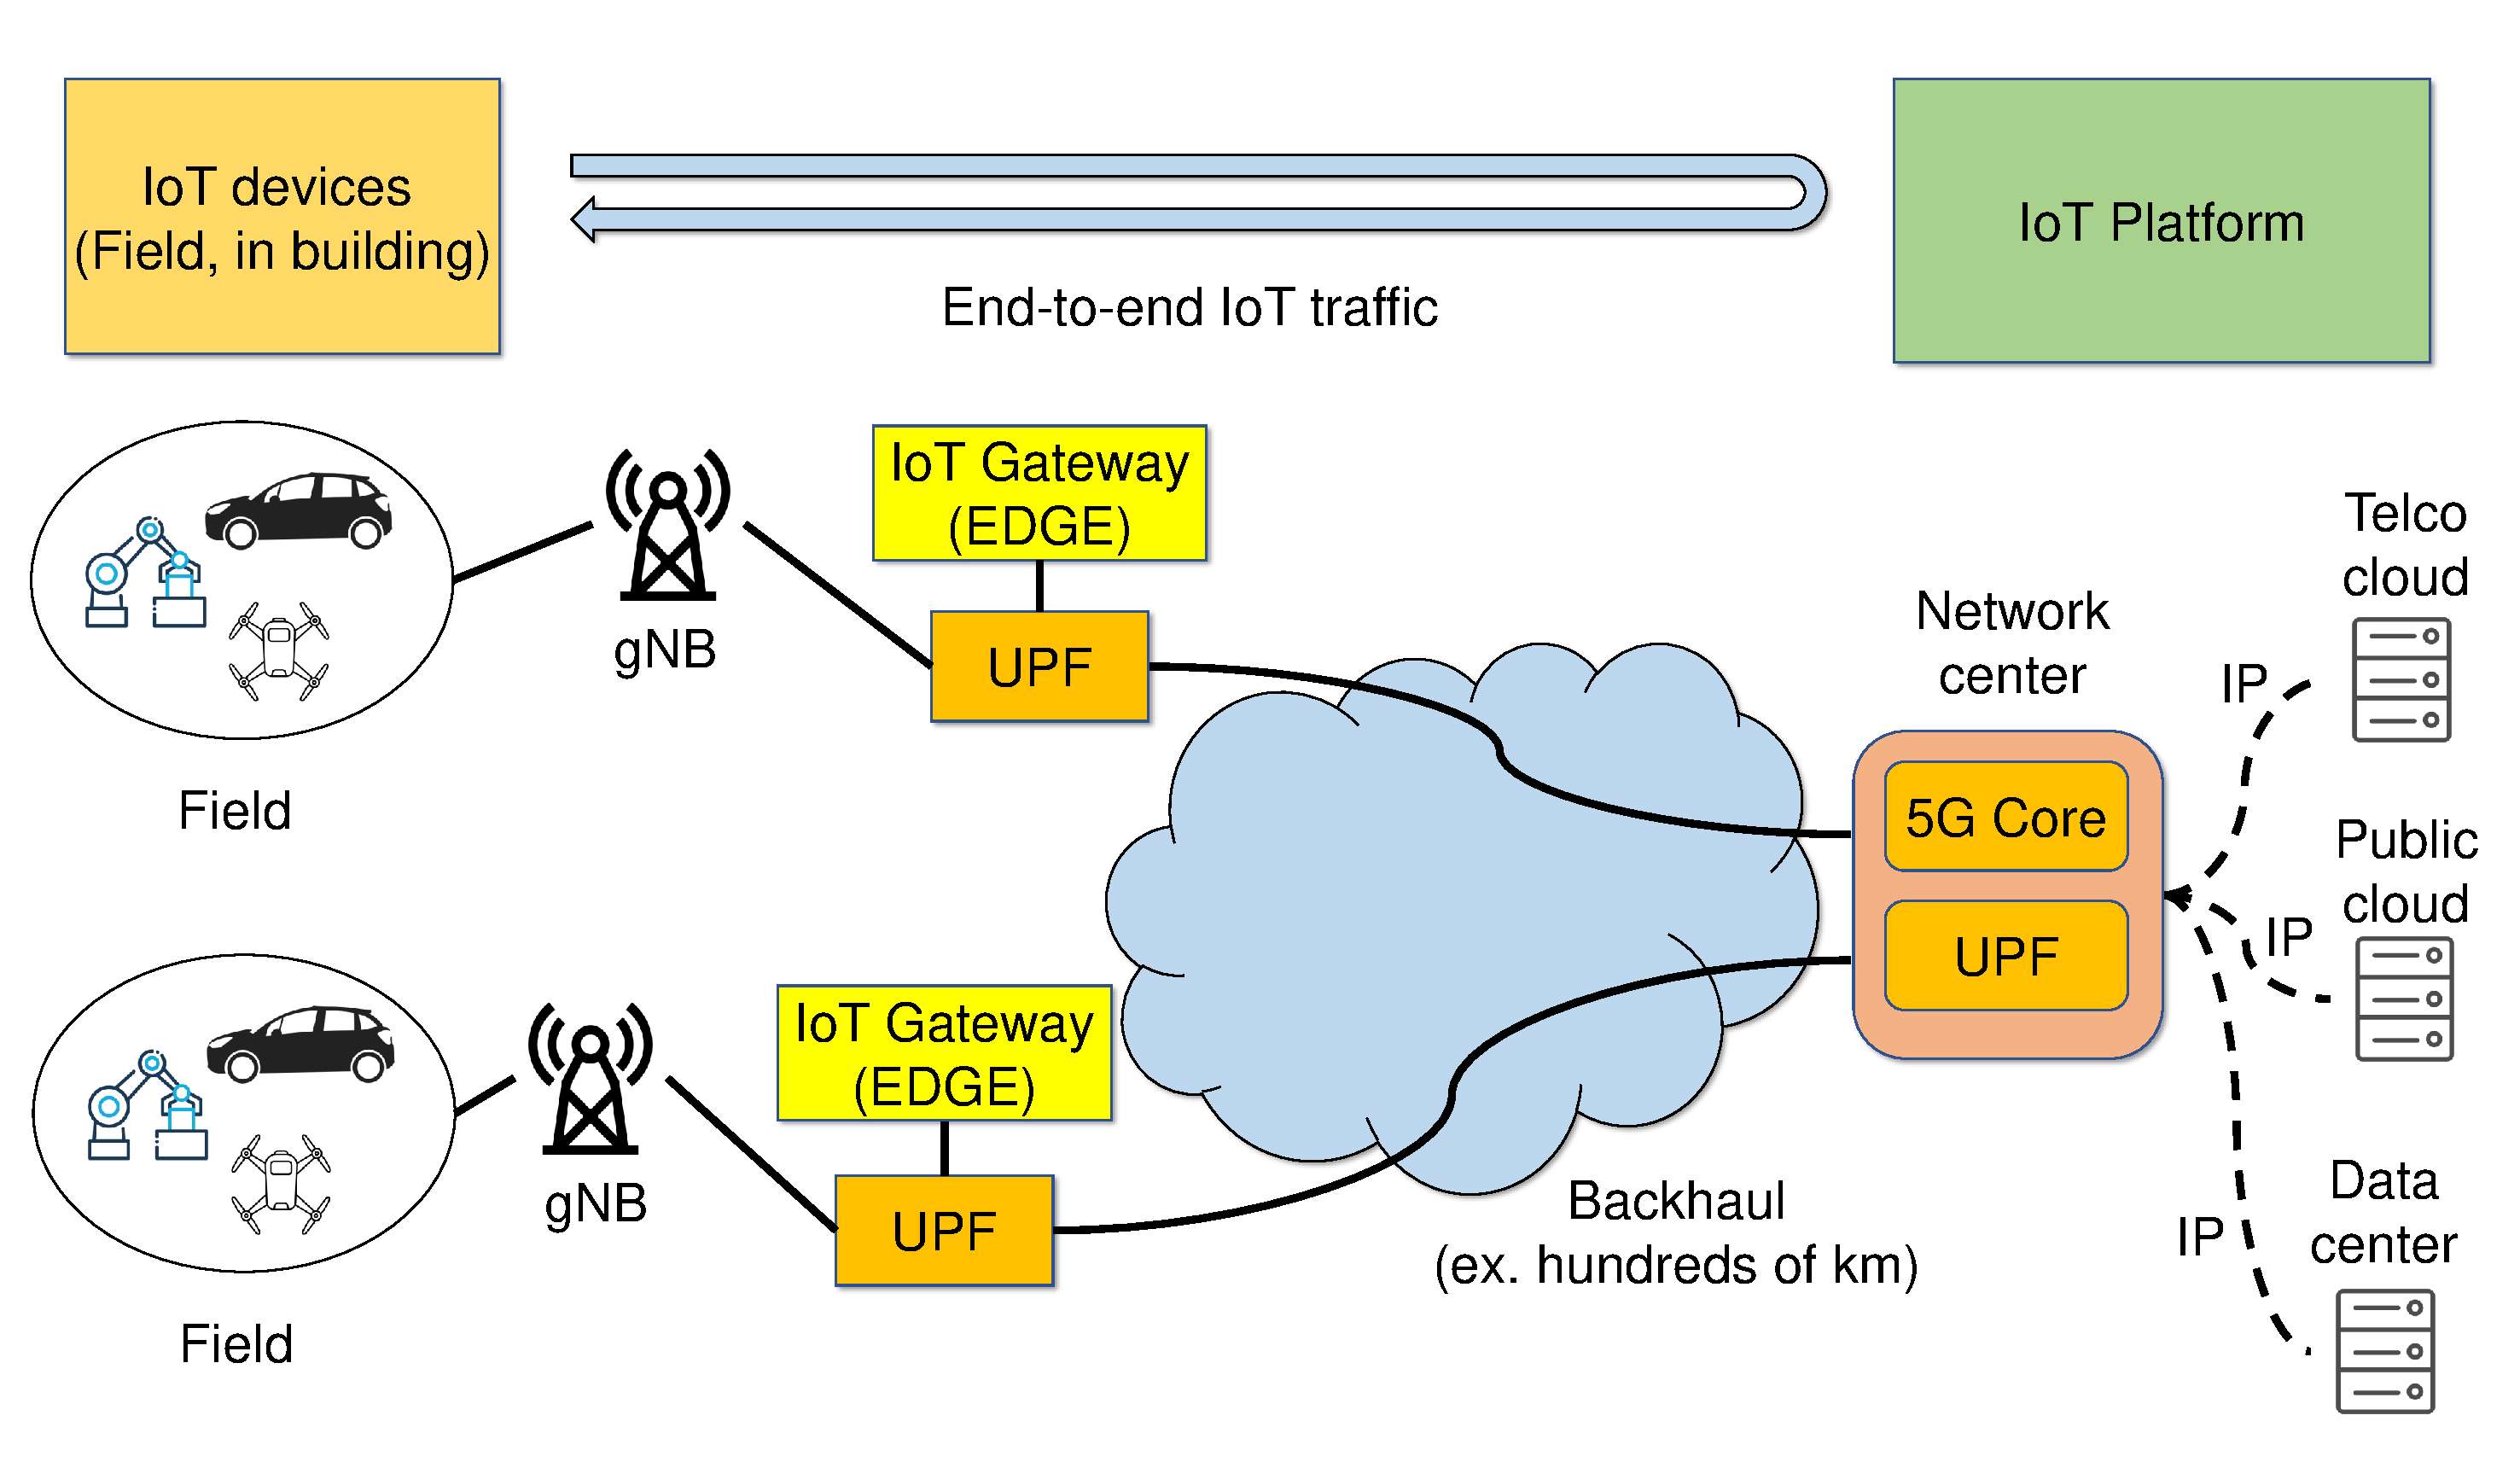
\includegraphics[width=\textwidth]{figures/fig_issue_of_current_network_slicing.pdf}
\caption{End-to-end traffic where IoT service platform is placed in the cloud}
\label{fig:network_slicing_issue}
\end{figure}

However, in order to fully make use of the advantages in the IoT service perspective, additional requirements must be fulfilled. For example, a cloud-based IoT platform where all common service functions are placed is typically fine to provide the smart home use case. In contrast, service providers need to consider much more different IoT use cases requiring more fast response time (e.g., less than a few ms) and higher reliability than other normal services; Industrial and mission-critical IoT services. In this situation, if the common IoT service functions are located far away from users, although the access and core networks are virtualized and move closer to the users, the request messages have to be reached to the cloud server, and IoT platform cannot serve the IoT services for the users within a few ms~\cite{husain2018mobile}. More specifically, as described Fig.~\ref{fig:network_slicing_issue}~\cite{edge_iot_netmanias}, when assuming network slicing is performed to the network infrastructure, the Round Trip Time (RTT) cannot be reduced since user's requests must reach the cloud-based IoT platform through backhaul in order to use IoT service that is launched far away from the users.

\subsection{Definition of IoT service slicing and task offloading}
A cloud-based IoT platform where all common service functions are placed is generally enough to support IoT services such as smart home and smart building use cases that do not require highly low latency. However, in other cases such as mission-critical IoT services based on less than a few ms, the existing IoT platform does not suitable since it cannot ensure fast response time to satisfy mission-critical IoT services requirements. 
In general, conventional IoT platforms are located at the cloud that is far away from the devices and applications. In addition, as the cloud IoT platforms provide all the required functions, if there exists a vast amount of data traffic from IoT devices, the resources on the cloud platform can be overloaded. Edge nodes can reduce such overload on the cloud via processing some or all data without transferring them to the cloud. Processing data at the edge node needs the edge nodes to support relevant IoT service functions. Take into consideration these requirements, a novel architecture for IoT service slicing and task offloading is introduced.

\subsubsection{MEC from the oneM2M perspective}
In the last few decades, mobile subscriptions have increased by up to 63\%, and a variety of new vertical services are being provided including videos, gaming, smart cities, smart factories and so on. In addition, the advancement of ICT forces the existing centralized cloud system to require very good performance. Therefore, to overcome the challenges in terms of latency and guarantee high speed, the ETSI MEC industry specification group~(ISG) has commenced developing standards including use cases, architecture, and application programming interfaces (APIs) to create an open environment and provide the vendor-neutral MEC framework~\cite{sabella2016mobile, taleb2017multi}.

\begin{figure}[tb!]
\centering
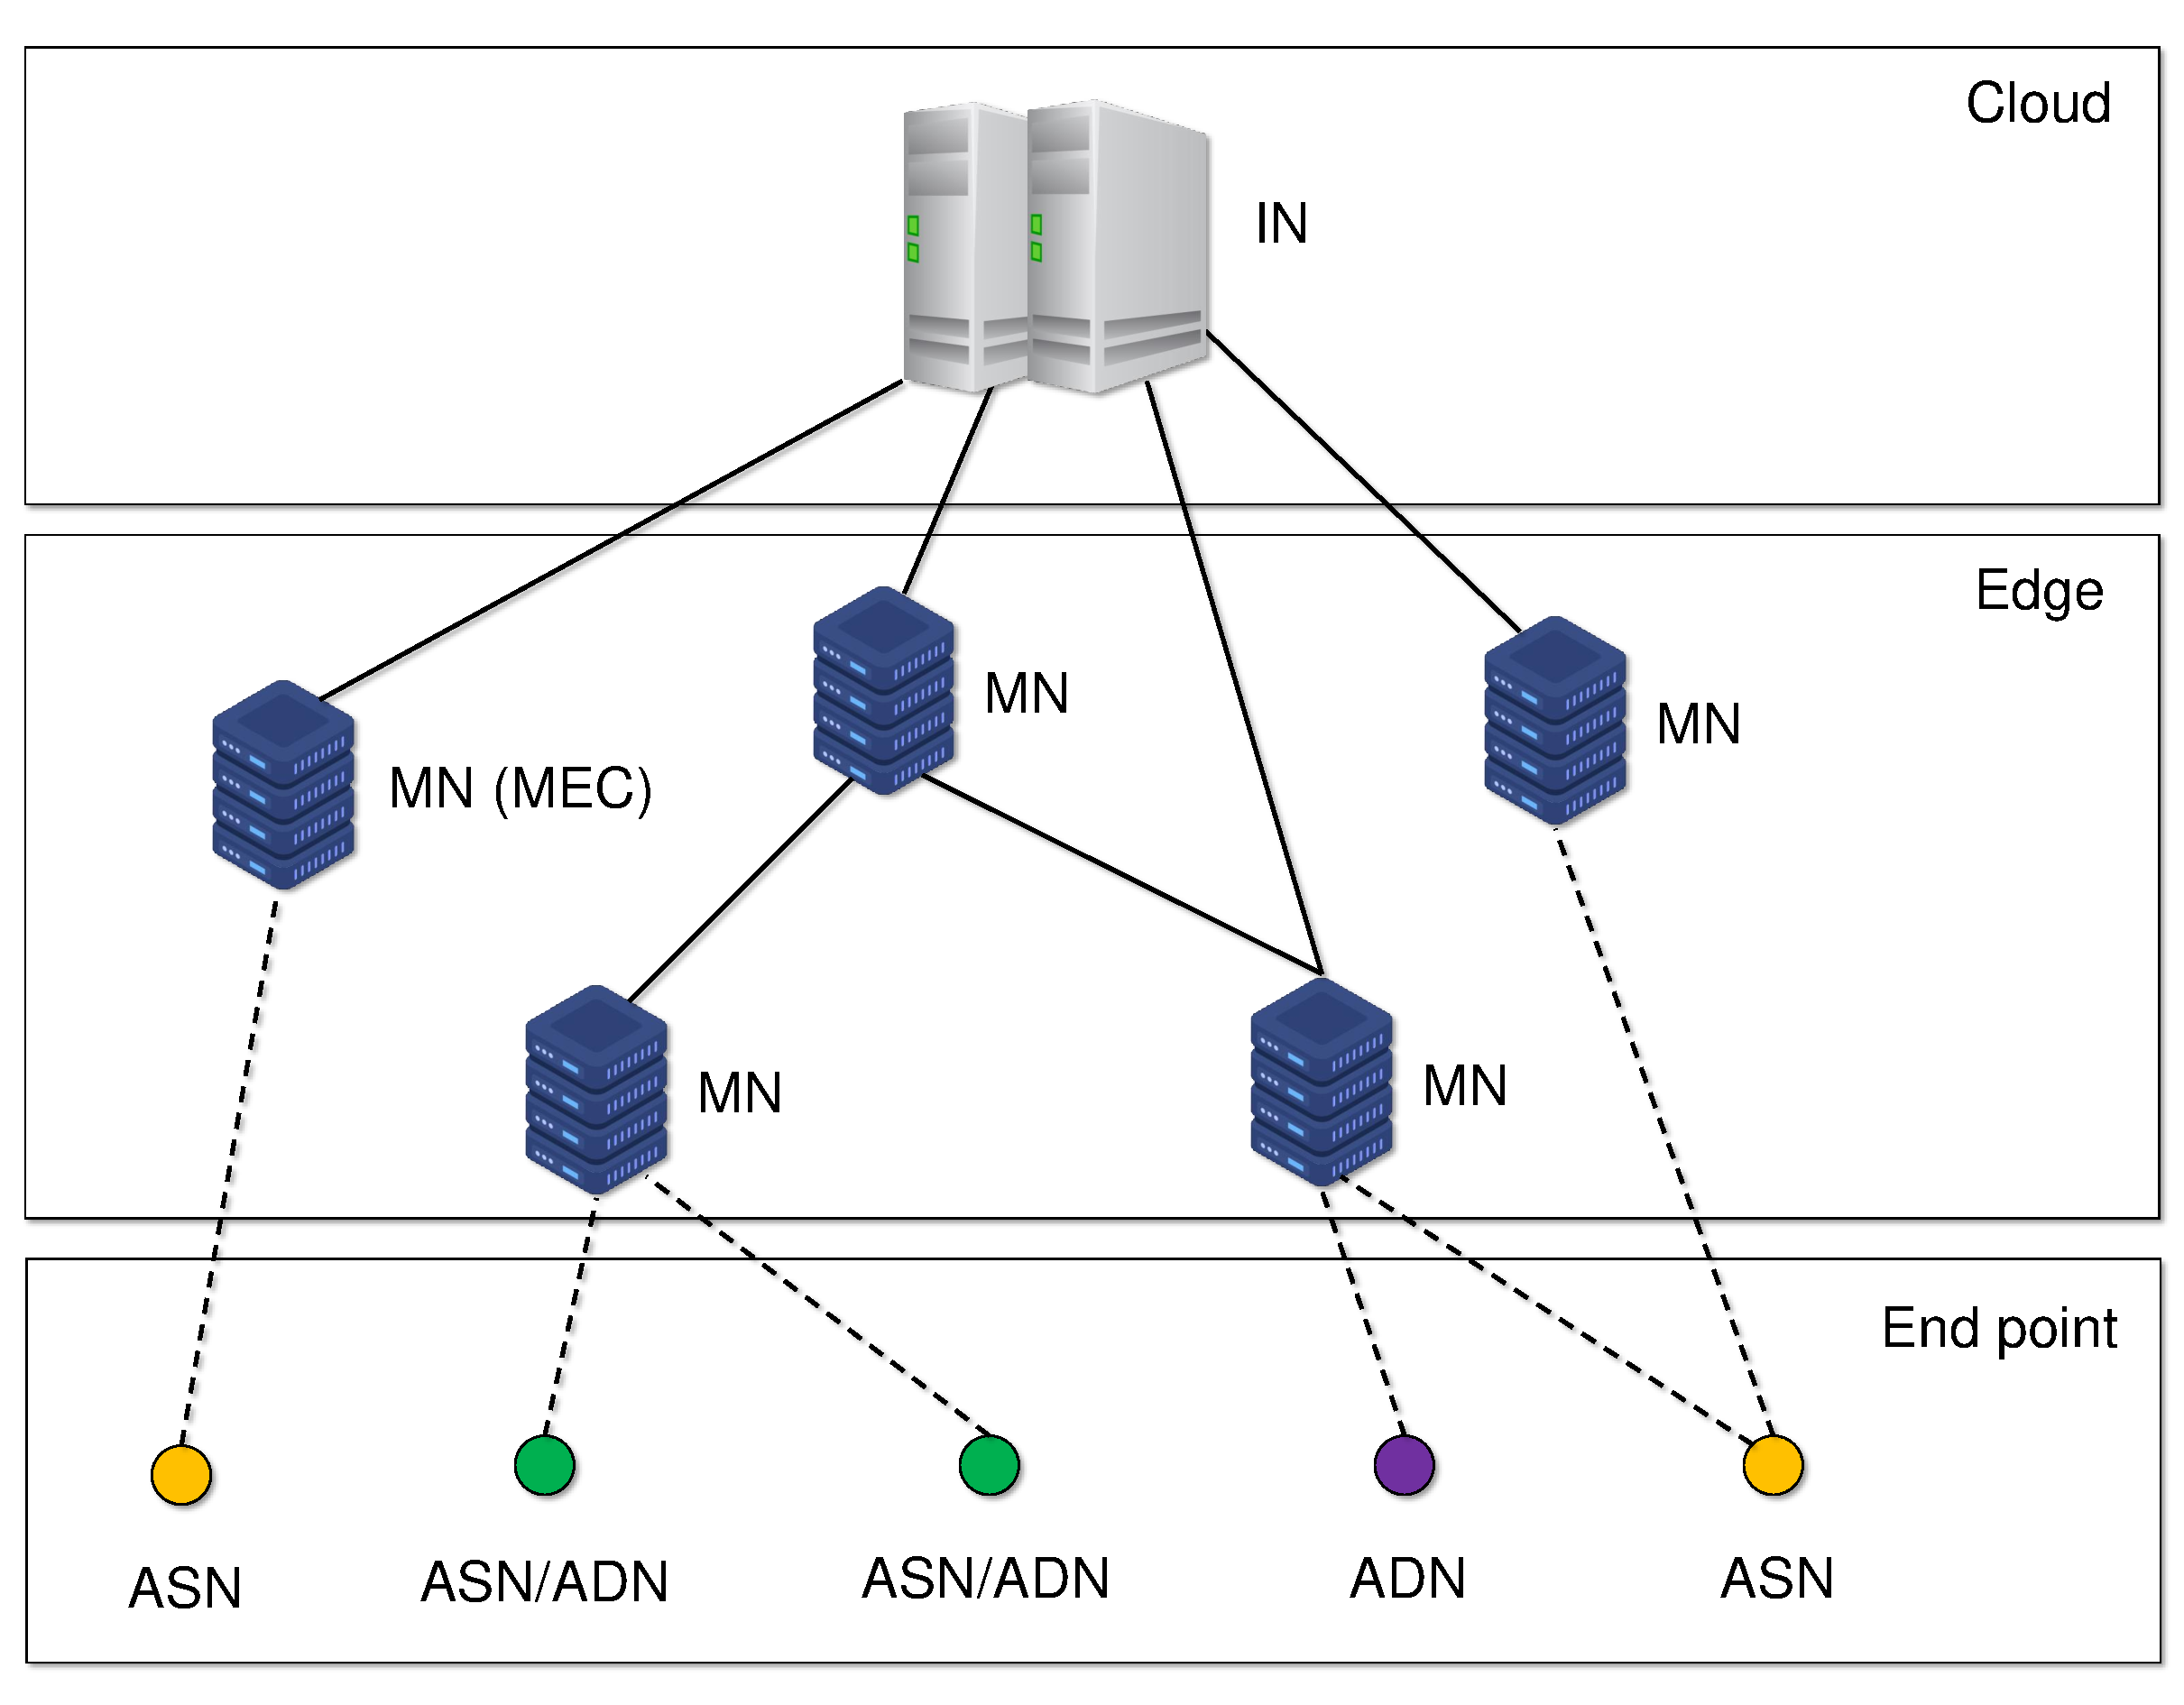
\includegraphics[width=1\columnwidth]
{figures/fig_IoT_slicing_onem2m_mec.pdf}
\caption{oneM2M reference architecture with MEC concepts}
\label{fig:onem2m_mec_perspective}
\end{figure}

According to the current oneM2M research regarding edge computing, one architecture model is proposed to integrate the MEC concept into oneM2M, and oneM2M sets the principle that the newly integrated edge computing concept has minimal impact on the existing oneM2M architecture~\cite {2020_onem2m_tr_0052}. In this context, the oneM2M node previously described can be presented as described in Fig.~\ref{fig:onem2m_mec_perspective}. The IN can be the cloud, the MN can be deployed either at the edge node or a normal gateway node, and the ADN and ASN can be the terminal devices. However, this conceptual architecture is not suitable for the full use of the current MEC architecture. Therefore, beyond simply applying the edge computing concept to oneM2M, the ETSI MEC ISG and oneM2M group are currently discussing how to provide an IoT-friendly environment by defining the MEC APIs for IoT systems.


\begin{figure}[tb!]
\centering
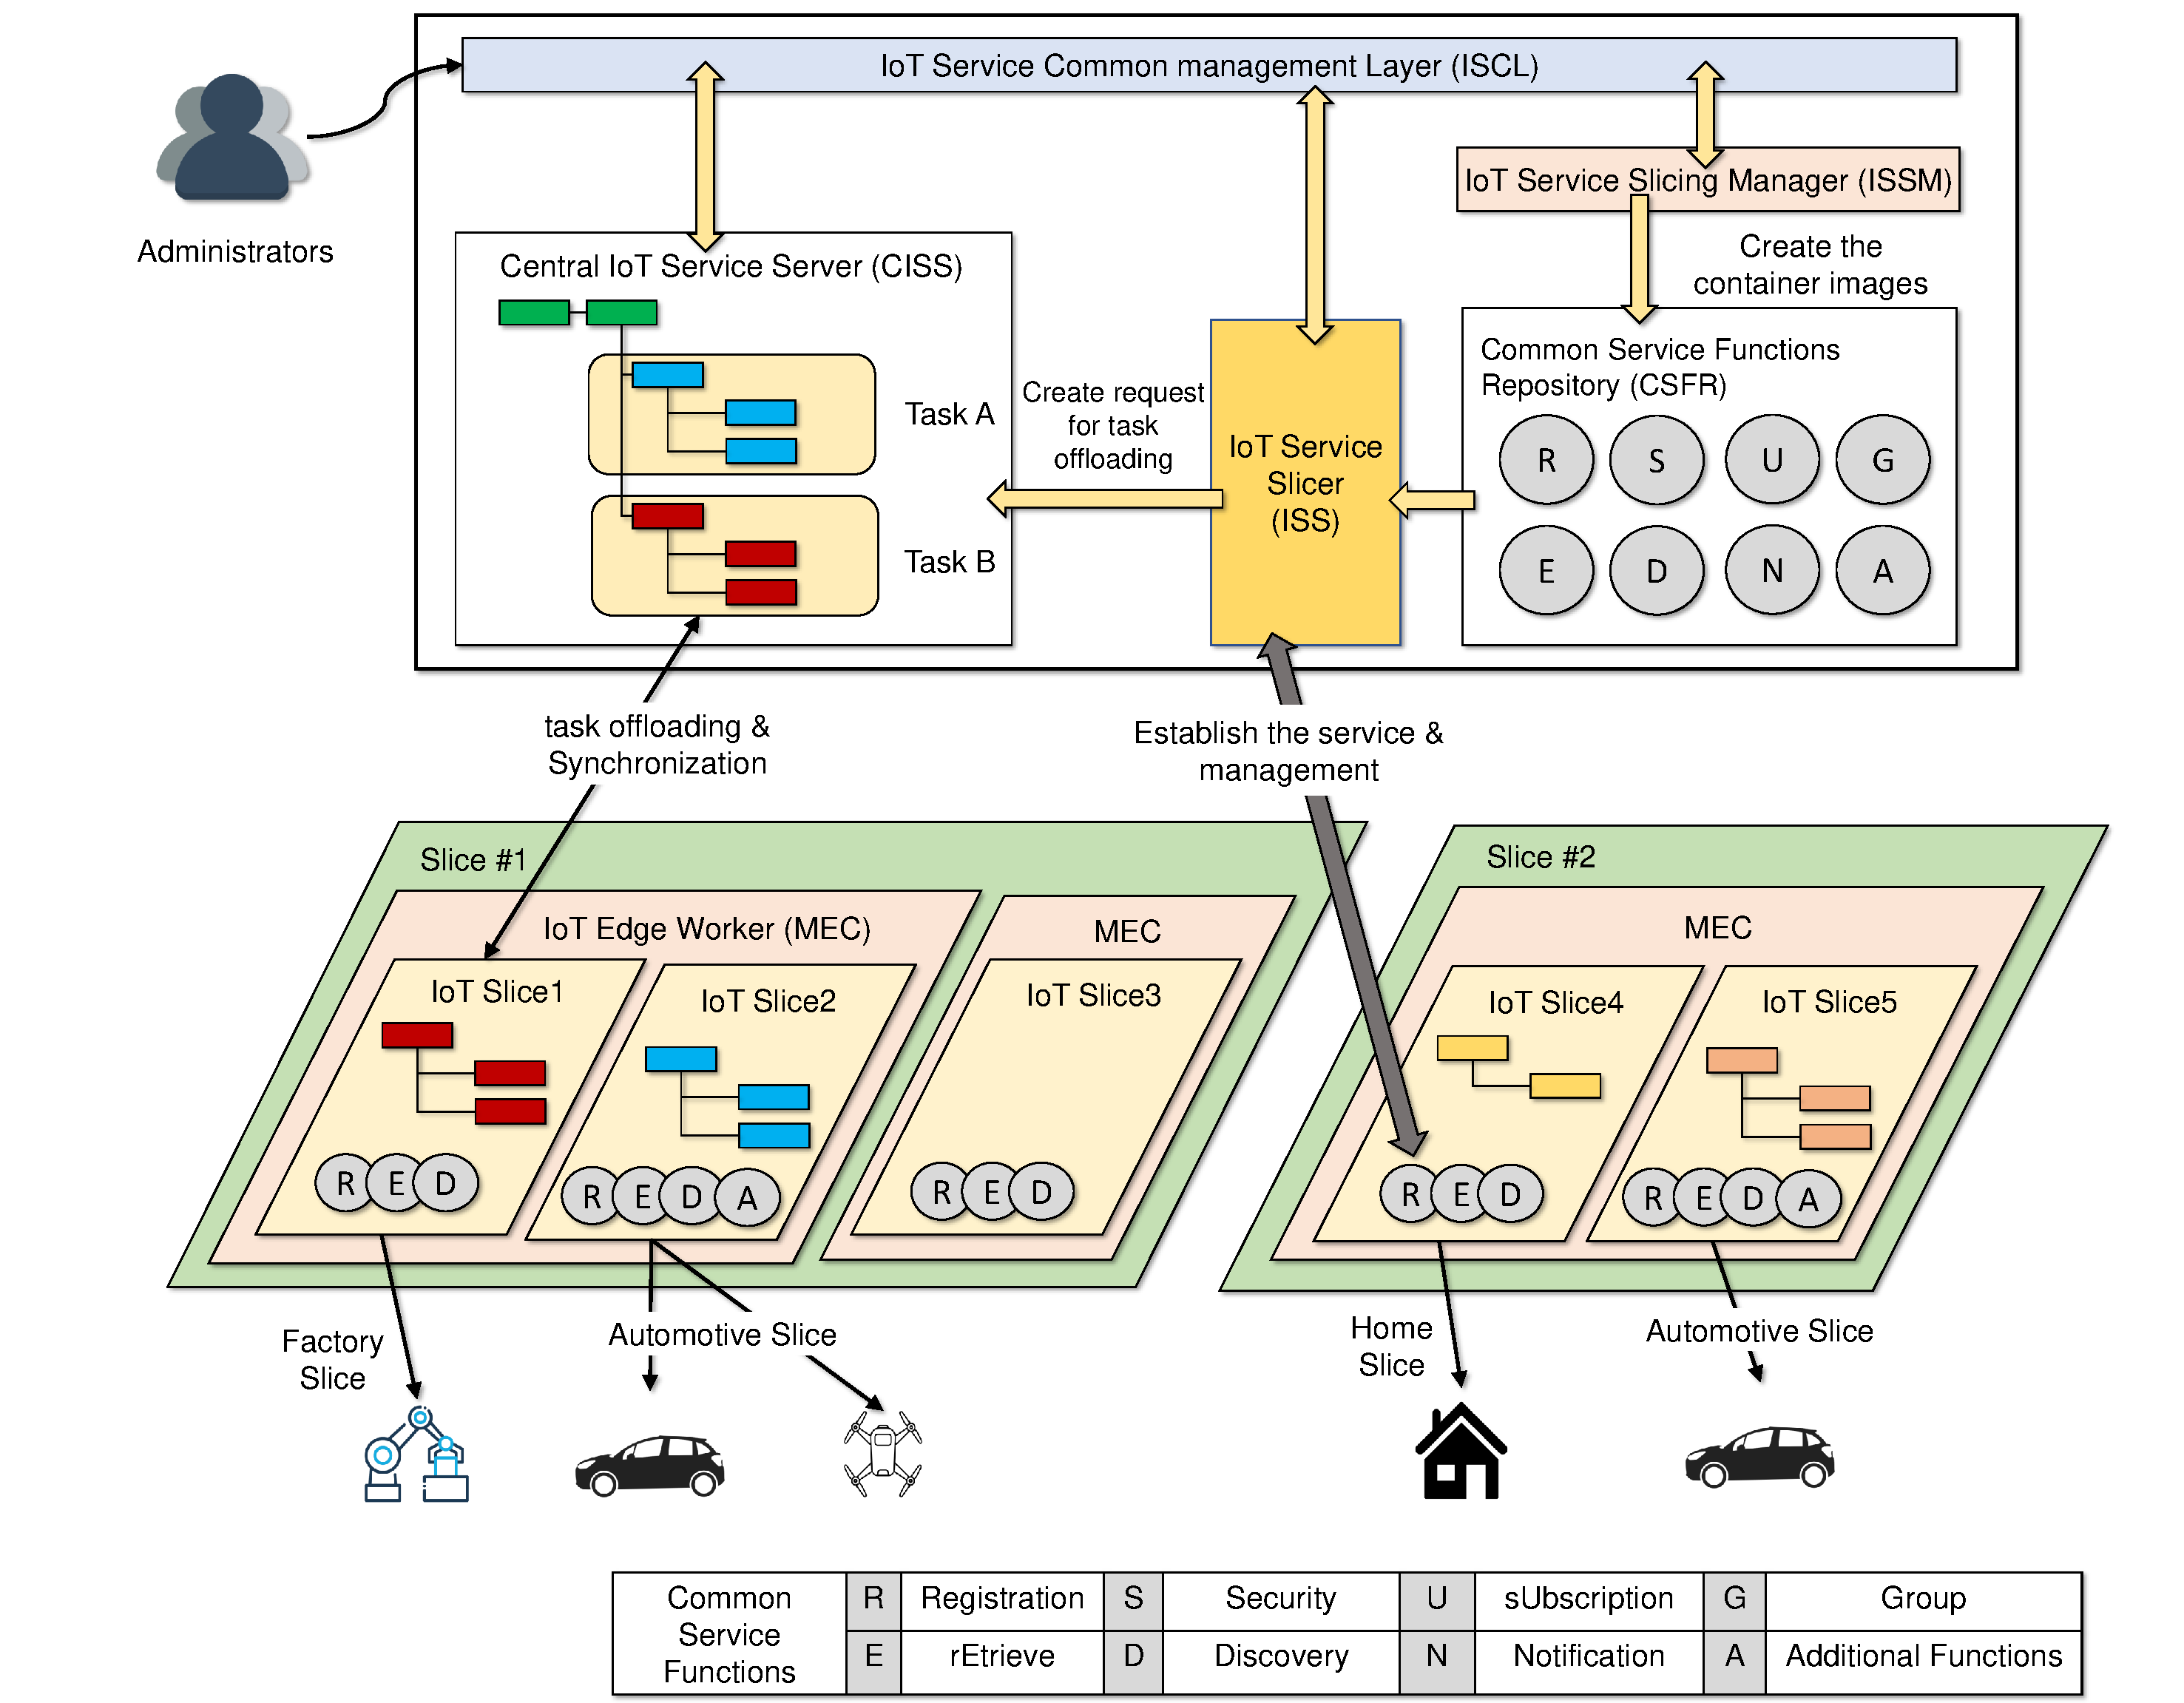
\includegraphics[width=\textwidth]{figures/fig_IoT_slicing_architecture.pdf}
\caption{Reference architecture illustrating IoT slicing and task offloading}
\label{fig:iot_slicing_architecture}
\end{figure}

\subsubsection{IoT service slicing}
IoT service slicing is a concept that modularizes the common service functions of the IoT platform into small microservices that can be deployed at the edge nodes. IoT service slicing selectively collects only necessary IoT microservices and creates a virtual IoT platform instance to move the instance towards the edge nodes. This allows the IoT system to operate IoT services more flexibly and efficiently so that each IoT slice can be optimized for a specific IoT use case. 

The proposed architecture comprises six logical entities to support IoT service slicing and task offloading as follows:

\begin{itemize}
\item \textit{IoT service common management layer (ISCL)} is a management layer that has entire views of IoT services currently operating in the cloud and an IoT service slicer that is responsible for slicing IoT services. Through this layer, administrators can understand the status of the currently running system through the logs.

\item \textit{IoT service slice manager (ISSM)} handles container-related requests from the ISCL. The ISSM is responsible for creating and storing the container images and has a collection of APIs for image management.

\item \textit{Common service function repository (CSFR)} is a repository to store container images for each IoT function. Basic IoT functions necessary for operating IoT services may be stored. In addition, according to specific requirements, additional components developed by the developer in accordance with the IoT platform standard may be stored in the CSFR. In this context, for example, Docker is used as a container technology. Docker uses a Docker image to run the container. Docker images are packages of application components required for each service, and since the configuration between each application is set in advance, they can be easily used in other new environments and are easy to manage and deploy~\cite{brogi2017dockerfinder}.

\item \textit{IoT service slicer (ISS)} is the orchestrator for processing both IoT service slicing and task offloading. The ISS initiates container images of edge nodes according to the IoT service types. In addition, the ISS delivers tasks to a specific edge node to provide IoT services at a short distance from users.

\item \textit{Central IoT service server (CISS)} can provide for all IoT functions in the cloud system and should have APIs between itself and each edge node to send commands and perform data synchronization. Therefore, the information processed at the edge node can be reflected in the IoT cloud to provide information through continuous updates. In addition, commands can be delivered through the cloud.

\item \textit{IoT edge worker} is the node that operates tailored IoT slices deployed by the ISS. The IoT edge worker is a \textit{container-runner} running on MEC and can support container-based software such as Docker. In addition, at IoT edge workers, containerized IoT functions are deployed and operated to support the IoT services of each user.
\end{itemize}

In this reference architecture, the microservice concept for IoT service slicing approach is decided to use. In general, deploying the IoT system at the edge nodes is not a relatively hard task if edge nodes have enough resources in terms of CPU, memory. However, providing the fine-grained graduality of IoT service based on the microservices gain more advantages from the perspective of resource management. First, a resource management perspective, when the IoT system is terminated due to unexpected errors, edge nodes do not need to respawn the container having a IoT system while if edge nodes adopt the microservices, it will just respawn the small-level microservices according to the IoT service type. For example, some simple IoT service use case such as measuring the temperature does not require subscription-notification IoT functionalities. In this case, the edge node does not need to load IoT systems having subscription and notification functionalities on the hardware. As a second reason, at the moment, there are many IoT services such as smart cities, smart factories and smart homes, and these IoT services may have different requirements in terms of latency, computation resources. In this regard, IoT services with different requirements can be operated on the same edge nodes. If all IoT services are being managed by the monolithic IoT system, each IoT service will have the same service level regardless of their requirements. In this context, for guaranteeing the Quality of Experience (QoE) of each IoT slice, classifying what IoT service is requiring more resources and assigning the resources to them is important. For example, a smart home service does not have a time-sensitive condition as a requirement. In contrast, mission-critical service such as medical, drone, smart car definitely requires the time-sensitive requirement and may make use of more resource than smart home services. In summary, classify the IoT service type and provide the IoT functions based on microservice is one of the promising options to operate the edge nodes efficiently. 

\subsubsection{IoT task offloading}
\label{sec:iot_task_offloading_procedures}

\begin{figure}[tb!]
\centering
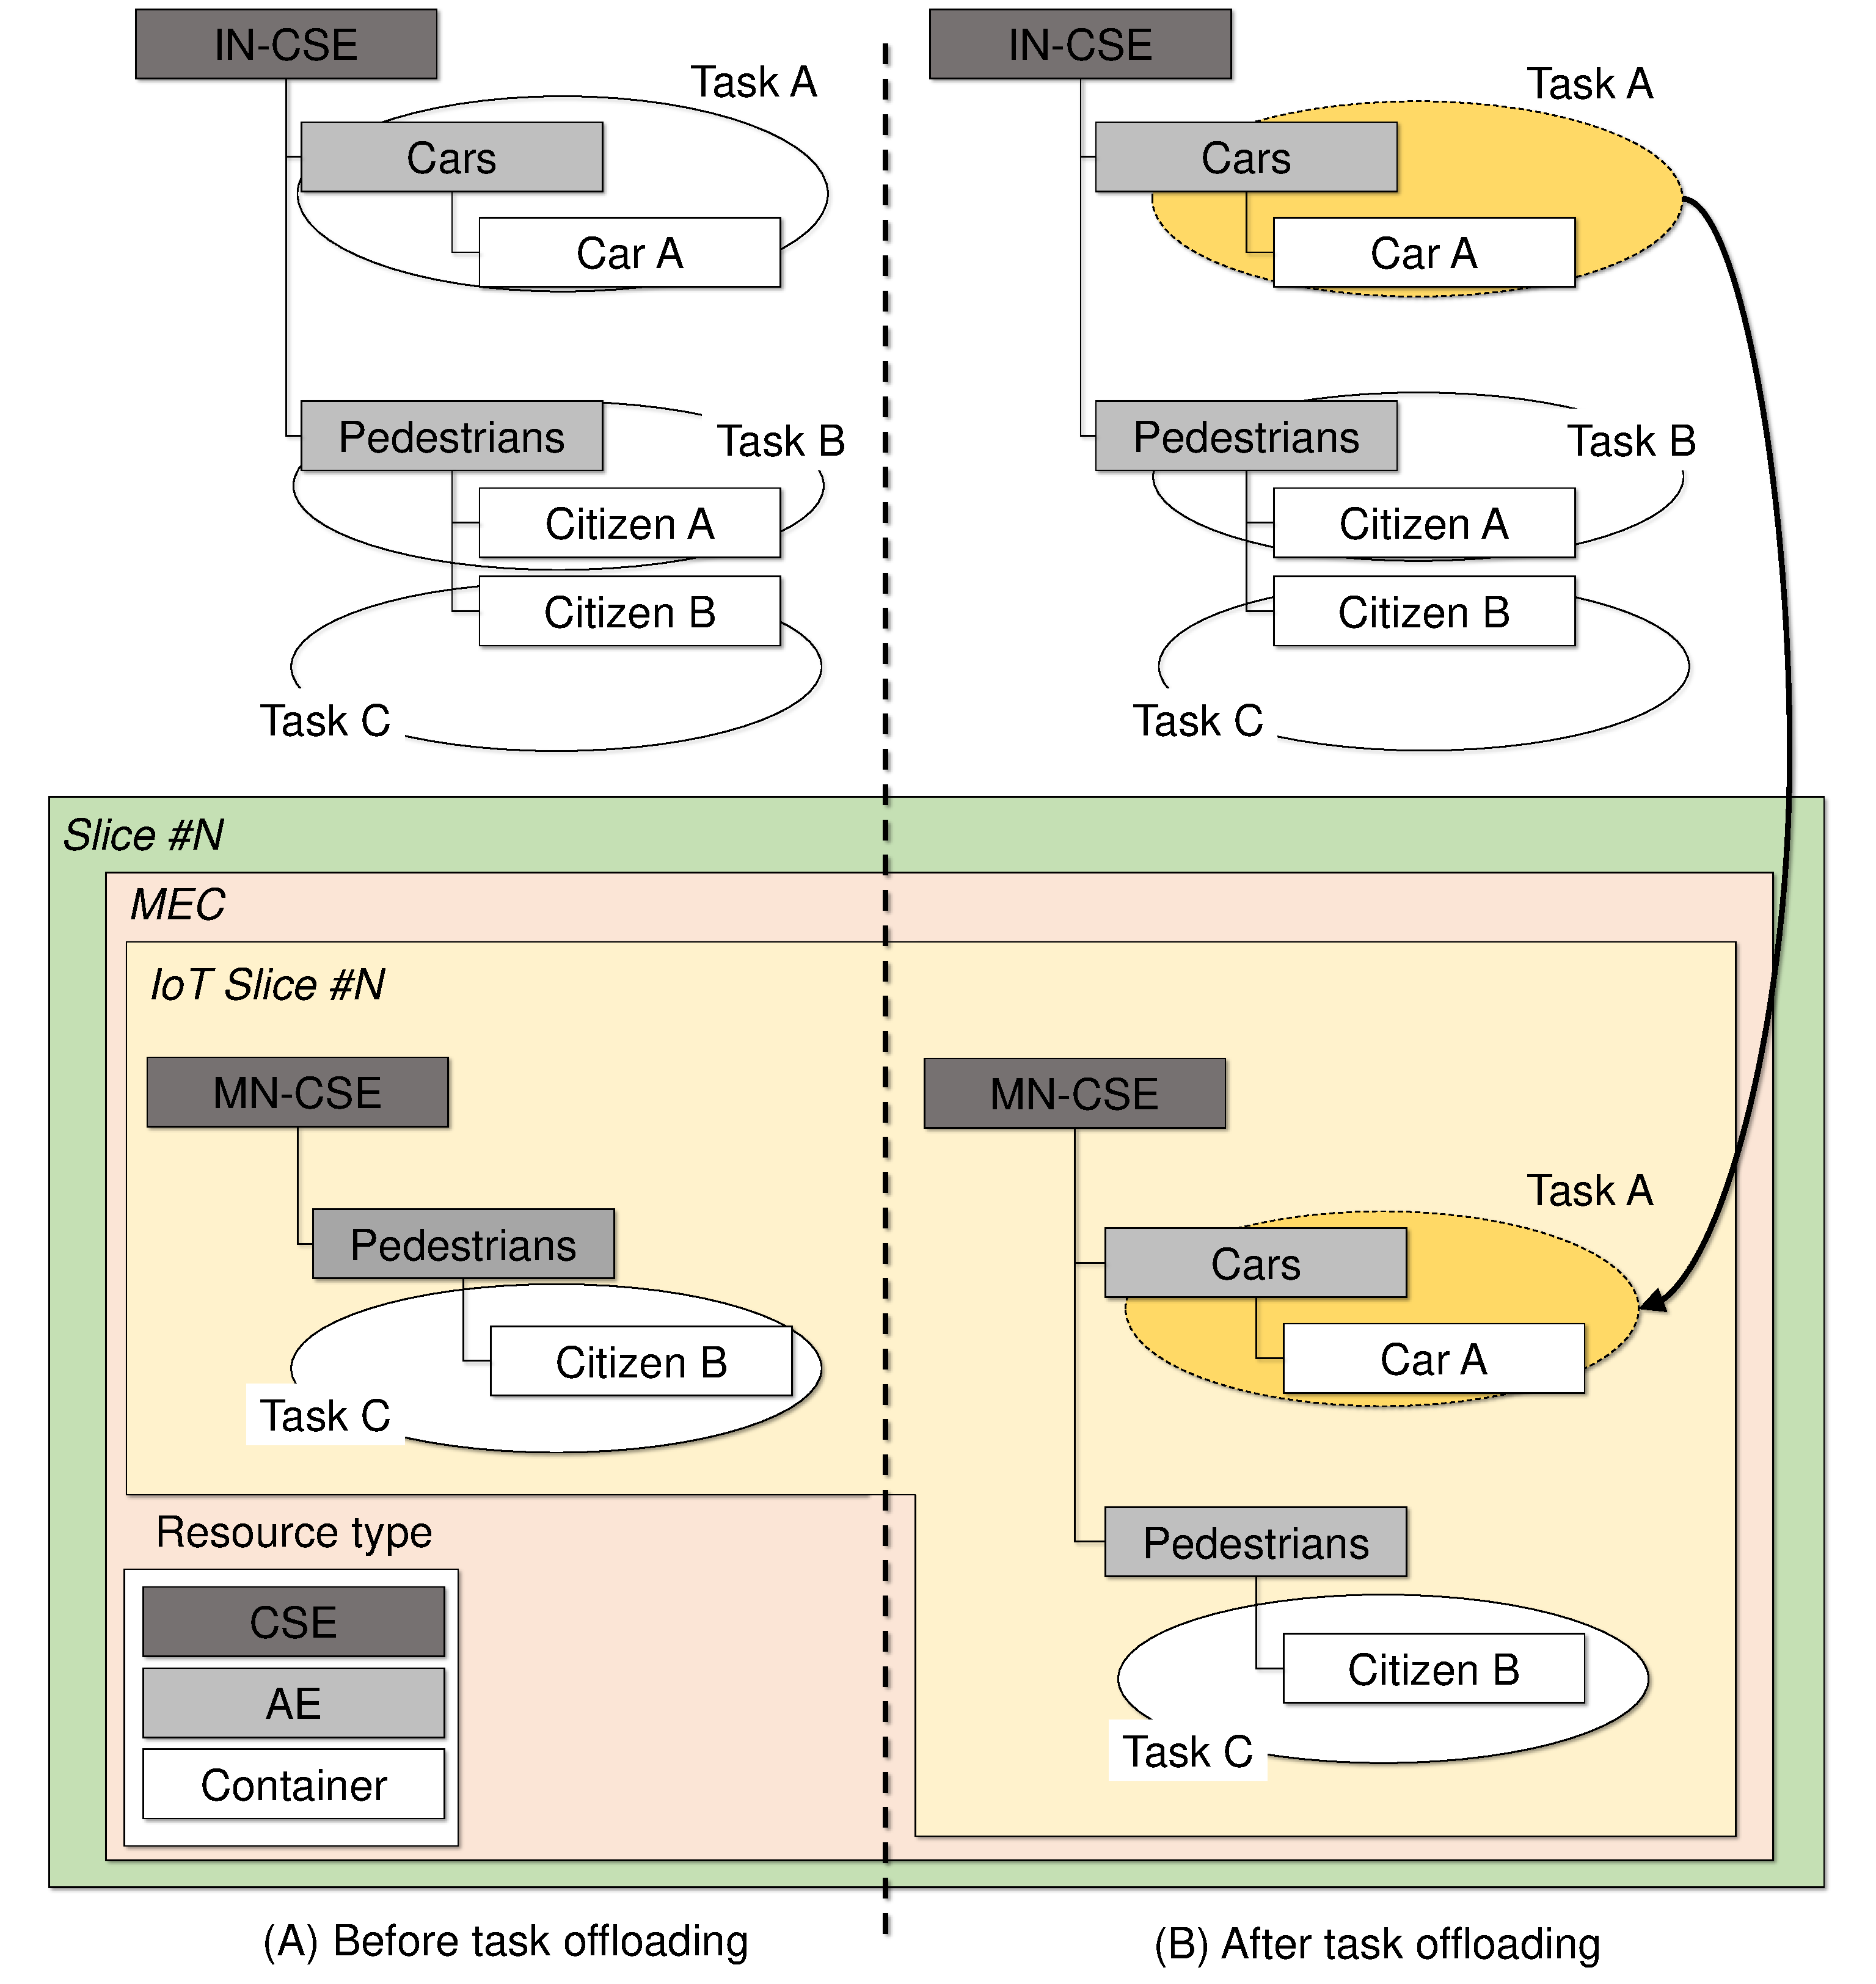
\includegraphics[width=\textwidth, height=12cm]{figures/fig_IoT_slicing_resource_offloading_edge.pdf}
\caption{IoT task offloading comparison}
\label{fig:iot_task_offloading_comparison}
\end{figure}

However, simply delivering the IoT functions to the edge nodes is not enough and, additional important procedures are left. IoT task offloading procedures copying the IoT resources into edge node are have to be considered. IoT task offloading is the transfer of IoT resources associated with the data to be processed at the edge nodes from the IoT cloud service platform. In IoT platform following ROA, as all IoT services are represented in the form of resources on the cloud, it is essential to have necessary resources on the edge node to mimic the requested IoT service.

That is, another important requirement for realizing IoT service slicing is not only to containerize IoT platform functions implemented in the cloud but also to deliver actual tasks to an edge node where the containerized IoT functions are instantiated. In this context, a task is a set of resources representing physical things and containing data and meta information on the IoT platform. Once the edge node is ready to serve a sliced IoT platform, relevant resources required to serve the service need to be placed on the edge node by IoT task offloading. As shown in Fig.~\ref{fig:iot_task_offloading_comparison}. (a), IoT physical entities are represented as a resource in the IoT platform. For example, a location of Citizen B is represented as a resource, \texttt{MN-CSE/Pedestrians/CitizenB/location}, in the edge node; the location is \texttt{<contentInstance>} resource and in order to serve service for other tasks by the edge node, relevant resources should be placed and managed in the edge node.

Let us consider a road scenario that warns the pedestrians crossing the crosswalk by sending the pedestrians' location to the vehicles. In Fig.~\ref{fig:iot_task_offloading_comparison}. (a), task A (IN-CSE/Cars/CarA/) and task B (IN-CSE/Pedestrians/CitizenA/) are running in the IoT platform of the cloud and another task C (MN-CSE/Pedestrians/CitizenB/)  is running at the edge node since Citizen B is walking in the smart city providing edge-based IoT services. When assuming task B is already offloaded and Car A on the highway is entering into the smart city if a request is made to use an IoT service with a few ms requirements by Car A, the IoT platform in the cloud must deliver the task being operated to the edge node. 
That is, in order to operate the service on behalf of the central cloud, the central cloud must offload the tasks being performed in the cloud to the edge gateway. After going through these procedures, the resource structure of task offloading is changed to the structure shown in Fig.~\ref{fig:iot_task_offloading_comparison}. (b). To recap, Car A can have more faster IoT services than before thanks to the shortening of transmission links. If the service is being served in the central cloud, hundreds of kilometers away, it could not meet the latency requirements for services. Therefore, the service such as road scenario, should be performed on the edge nodes near the services.

\subsection{IoT service slicing and task offloading procedures}
This subsection describes the procedures of how to achieve the IoT service slicing by performing IoT function modulization, and task offloading based on the container technology and IoT standards. Detailed procedures for IoT service slicing and resource offloading are described based on MEC and oneM2M global standards~\cite{marques2019internet, 2020_onem2m_tr_0052}. 

\begin{figure}
\centering
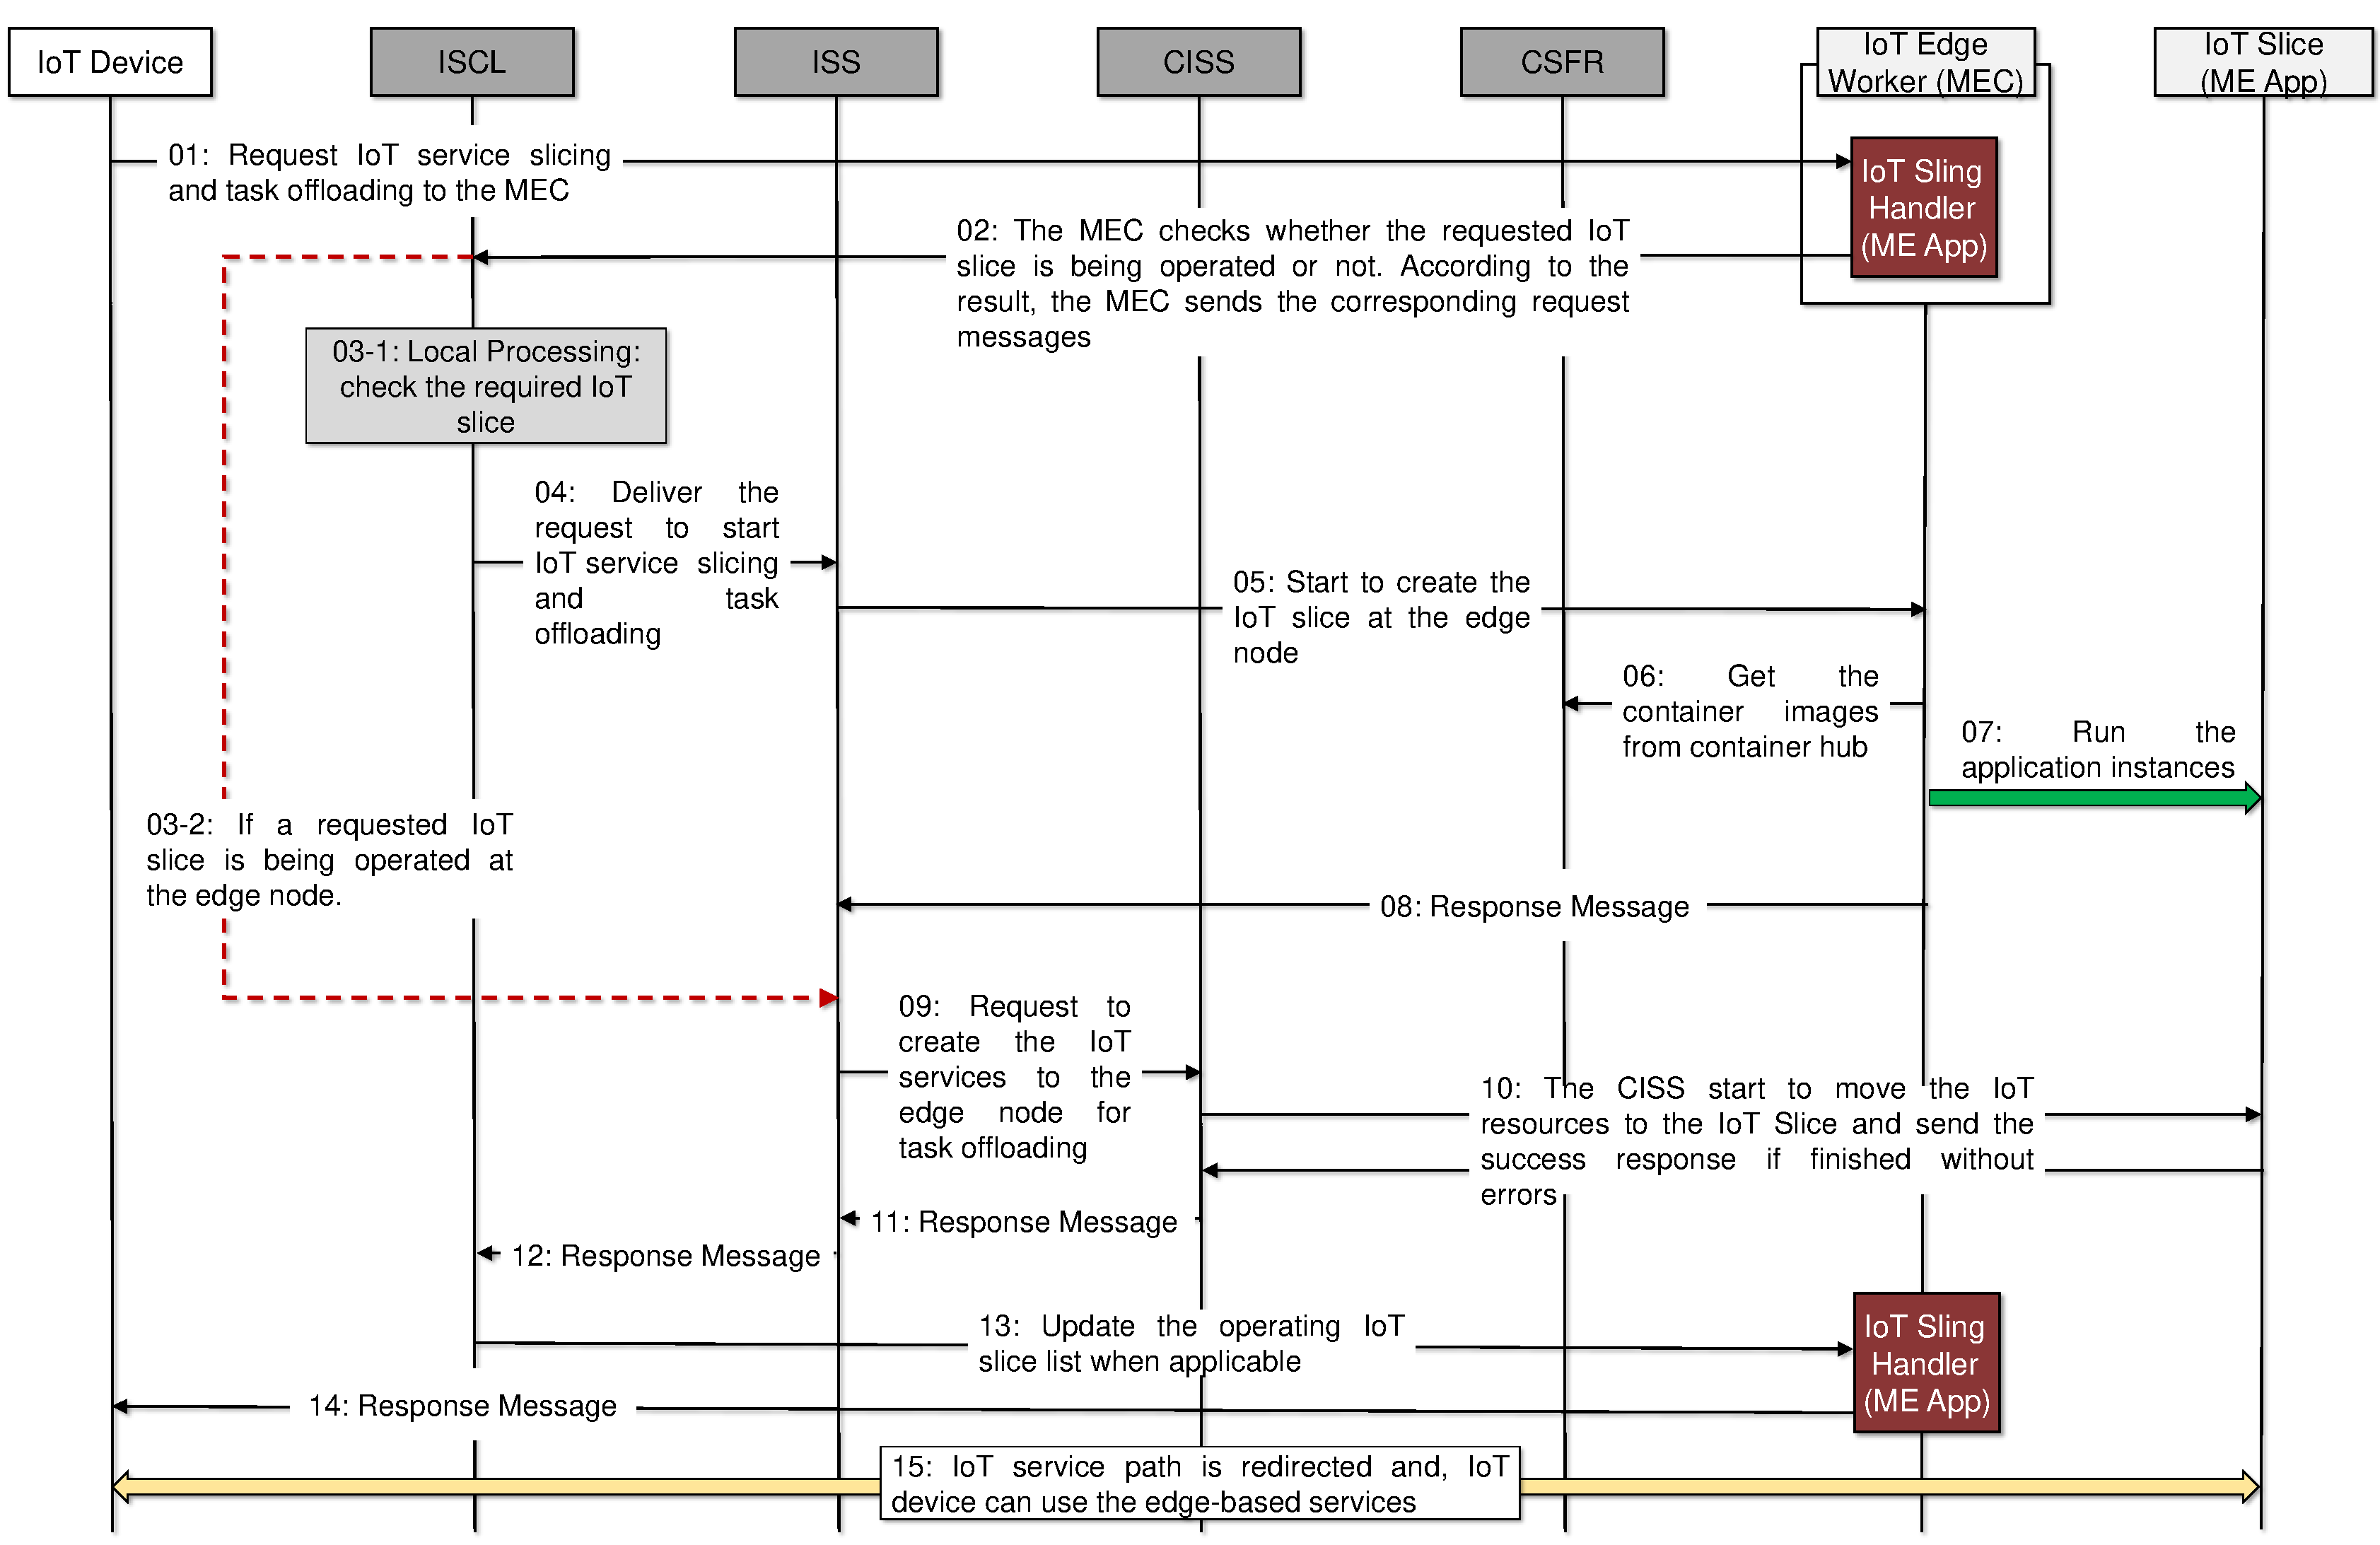
\includegraphics[angle=90, width=1\textwidth]
{figures/fig_IoT_slicing_resource_slicing_procedures.pdf}
\caption{IoT service slicing and task offloading initial procedures}
\label{fig:iot_task_offloading_procedures}
\end{figure}

\subsubsection{Detailed procedures for IoT service slicing and offloading} In these procedures, according to the IoT devices' request, first, IoT slicing is executed to provide the IoT functionalities to the edge nodes~(steps 01-08). Next, IoT task offloading is performed to deliver the already operational IoT services in the central cloud to the edge nodes~(steps 09-14). These procedures are materialized by using the components that we described above, and three main components, namely, ISSM, CISS, and ISS, are used.

\begin{enumerate}
\item [01:] IoT devices send a request to the MEC node to use edge-based IoT services. In this context, IoT devices can be mobile phones or many other devices based on the Internet such as drones or smart cars.

\item [02:] In the MEC specification~\cite{computing2019framework}, the ME App (MEC Application) that is running as virtual machines on top of the virtualization infrastructure is defined. In this article, the ME App can be an IoT slice with IoT function container instances. In addition, the IoT Slicing Handler, also an ME App, is defined to address IoT-related messages. More specifically, the IoT Slicing Handler is deployed in advance to act as an IoT message handler and holds information about the instantiated IoT functions per IoT slice that are currently being performed. Based on this information, the IoT Slicing Handler matches the request from the IoT device and checks whether required IoT functions for a requested IoT slice can be supported by currently running IoT slices. According to the matching result, the IoT Slicing Handler delivers a corresponding request message to the ISCL.

\item [03-04:] The ISCL is responsible for structuring the request message for the ISS and sends the message with information such as IoT service information, necessary IoT functions, and target edge node information. 
If the ISCL receives a message that indicates the required IoT functions are already supported by one of currently running IoT service slices, it delivers the IoT task offloading start message to the ISS (step 03-2, Go to step 09) by omitting steps 4-8 (for performing IoT service slicing). 
%If the ISCL receives the message not including IoT function generation from MEC, it delivers the IoT task offloading start message to the ISS (step 03-2, Go to step 09) by omitting steps 4-8. 
In contrast, in case some of the requested IoT functions are not performed by one of IoT slices, the ISCL delivers an ``IoT function generation and task offloading" message to the MEC (steps 03-1, 4).

\item [05:] The MEC defines data models and related procedures as well as various APIs based on REpresentational State Transfer (REST) to provide the edge computing services~\cite{sabella2019developing}. 
For instance, there is an API to check whether the MEC App instance operated in the MEC system is currently running (\textit{MEC application support API}~\cite{computing2019enablement}) and a procedure to initiate or terminate a specific MEC App instance (\textit{application instance lifecycle management}~\cite{computing2019management}).
Therefore, the ISS exchanges information with the MEC to provide IoT services using these various MEC APIs and related procedures.
The ISS sends the message to start creating a required IoT slice to perform requested IoT service functions that are not supported by the existing IoT slices on the edge node.

\item [06-08:] In this phase, if the IoT edge worker already has the container images regarding the IoT functions that are not currently running, then that service function is simply initiated.
Otherwise, the IoT edge worker has to access to the CSFR to download the required IoT service container images (step 06). After downloading the required container images, IoT edge worker initiates the containers to provide IoT functions (step 07). After confirming that all containers have been deployed to the edge node, the deployment phase of the IoT function for IoT service slice is finished, and now, the edge node can be considered as having an operational ``IoT slice (ME App)" (step 08). 
For reference, since the MEC standard is currently based on a virtual machine~\cite{computing2019virtualisation}, it does not download images from a specific image hub when there are no images. That is, MEC previously stores related images before initiating an application through a procedure such as an \textit{application package management procedure}. However, this article describes the procedures under the assumption that MEC is used on a container basis~\cite{computing2019management}.

\item [09-12:] For IoT task offloading, an IoT task offloading request message is sent out into the CISS with the IoT service information of a user (step 09). 
The CISS delivers tasks and data that are running and stored in the cloud to edge nodes to provide the edge nodes with IoT tasks that are currently supported in the cloud (step 10). 
The edge that receives the information can create IoT tasks to an IoT slice running on the edge node itself to seemingly perform the IoT service within a short distance from the user. 
In addition, the additional API should be defined not only to synchronize the data between the IoT slice at the edge node and the cloud but also to deliver the command or exchange the data with the cloud. 
When all tasks running in the existing cloud are deployed to the IoT slice at the edge node, the edge gateway is finally ready to support the ``proximity of IoT services" (step 11). 
When the ISS sends the response message to the ISCL, it includes the list of the newly initiated IoT functions of the IoT slice (step 12).

\item [13-14:] In these steps, if the IoT service is newly initiated or some IoT functions are newly initiated in the existing IoT service slices in steps 05-07, this information is reflected by the IoT slicing handler. Therefore, later, if the IoT device requests the same IoT service, the IoT slicing handler can aware that the existing IoT slices support required IoT service functions and will just request IoT task offloading.

\item [15:] After performing all the previous steps, IoT devices can directly receive required IoT services from the edge node providing IoT service slicing and task offloading.
\end{enumerate}

\subsubsection{IoT task offloading synchronization} As mentioned in the CISS component description, an additional API is needed to synchronize the information between edge nodes and the central IoT platform. 
More specifically, although the data generated by the IoT devices are stored in the edge node, if these data are not synchronized with the database of the IoT platform existing in the cloud, IoT applications that are not using the IoT service slicing cannot use the latest updated information. 
Accordingly, all data stored or updated at the edge node must be synchronized with the data managed by the IoT platform existing in the cloud. 
To realize synchronization, the ``subscription-notification" mechanism can be considered as a suitable method. 
The IoT platform subscribes to specific task offloaded resources of the edge node so that the IoT platform can receive the updated contents from the edge nodes whenever there exist any updates. 
If the data of the subscribed resource are changed (e.g., updated with a new value or deleted), the edge node generates a notification message including the information about the changed data and delivers it to the IoT platform. 
The IoT platform that receives the notification can analyze the messages and update the corresponding data in the cloud to be synchronized with the one in the edge node. 
For example, in the oneM2M IoT standard, there is a \texttt{<subscription>} resource, and this resource can be created under specific resources to check any changes of the resource as described in subsection~\ref{subsec:onem2m_overview}.
When the status of the subscribed resource changes, the edge node checks the notification target uniform resource indicator (URI) and sends the changed information to the IoT platform. 
As a next step, the IoT platform updates the changed information to synchronize.

In addition, another synchronization approach can be considered. 
Among IoT service use cases, there might be a case such as measuring temperature in a building. 
In this case, data can be delivered to the IoT platform over a relatively long period since the temperature does not change often. 
In contrast, another use case such as smart cars and drones can generate the data rapidly and frequently, and they would produce massive quantities of data within a short time period. 
The former case can use the synchronization method mentioned earlier. 
However, the latter case can degrade the performance by continuously creating and transmitting a synchronization channel, which results in using many resources on both the edge node and cloud. 
Therefore, if the task offloaded resource at the edge node is updated, immediate synchronization better not be occurred in the latter case. 
Instead, when retrieve requests arrive at the cloud from the IoT applications, the cloud can redirect the service path to the edge node where an active IoT slice for the requested service is currently running. 
For instance, when a retrieve request for a specific resource is delivered to the cloud, after checking the existence of an IoT slice associated with the resource, the request is delivered to the edge node that runs the IoT slice. 
Then, the data most recently stored or updated are delivered to the IoT application. 
In this case, synchronization can be performed after the termination of the IoT service running in the edge node. 
%To summarize, with these examples, we defined the ways to synchronize both the edge node and cloud. 
%However, this is not the absolute case, which means that approaches can be different according to the operating environment conditions.
As there exist many different scenarios, a proper synchronization mechanism can be different according to the operating environment conditions. 

To demonstrate the advantages of IoT service slicing and task offloading in the subsequent section, a Docker-based IoT service slicing environment to perform function distribution and resource offloading is implemented.

\subsection{Experimental evaluation}

To prove the advantages of our proposed IoT slicing and task offloading, this subsection uses oneM2M standards and implements the IoT platform based on microservices using Docker to perform container-based IoT function orchestration and IoT task offloading. 
Based on this implementation, performance comparison of the latency between the IoT services running on the central cloud and those using the sliced IoT functions in the edge gateway is conducted.

\subsubsection{Experimental setup and Implementation}
To evaluate the impact of the proposed IoT slicing concepts, Docker, which initiates the container images in the devices, is used to make the testing environment as described. 
In addition, to compare the performance before and after IoT service slicing and IoT task offloading, as shown in Fig.~\ref{fig:iot_service_slicing_environment}, two scenarios are conducted: a cloud-based IoT service (blue line) and edge-based IoT service (red dotted line). 
Figure.~\ref{fig:iot_service_slicing_environment_edge_detail} provides detailed information on how IoT microservices are deployed and operated at each edge node. 
In this scenario, it is assumed that the edge node is capable of operating a Docker-based service and that the container images for executing IoT microservices are already deployed. 
For example, container images such as Registration (R) and rEtrieve (E) are already deployed at an edge node, and accordingly, the edge node can initiate these images without accessing the Docker Repository Hub. 
IoT microservices to perform a specific IoT service can be arranged with Registration (62590), Retrieve (62591), Subscription (62592), and Notification (62593), and numbers in parentheses indicate the port number on which each microservice operates. 
In addition, each IoT microservice operates on the HyperText Transfer Protocol (HTTP). 
To focus on the performance and low memory, these IoT microservices are developed based on the Node.js Web framework, which is a server-side JavaScript environment~\cite {tilkov2010node}. 
The series of procedures for interacting with microservices are executed based on the Docker Remote Engine API, which provides an API for interacting with the Docker daemon~\cite {DockerEngineAPI}. 
The IoT task offloading procedure is the same as that described in section~\ref{sec:iot_task_offloading_procedures}, and additional considerations for edge nodes and the IoT platform are how to synchronize the data change between them. Therefore, after IoT task offloading, 
as described in Fig.~\ref{fig:oneM2M_resource_structure}, the \texttt{<subscripton>} resource is created under each \texttt{<container>} resource to check the status change such as data update.
If data are updated at the edge node, a notification message is automatically configured and sent to the IoT platform to perform the data synchronization.

\begin{figure}[tb!]
\centering
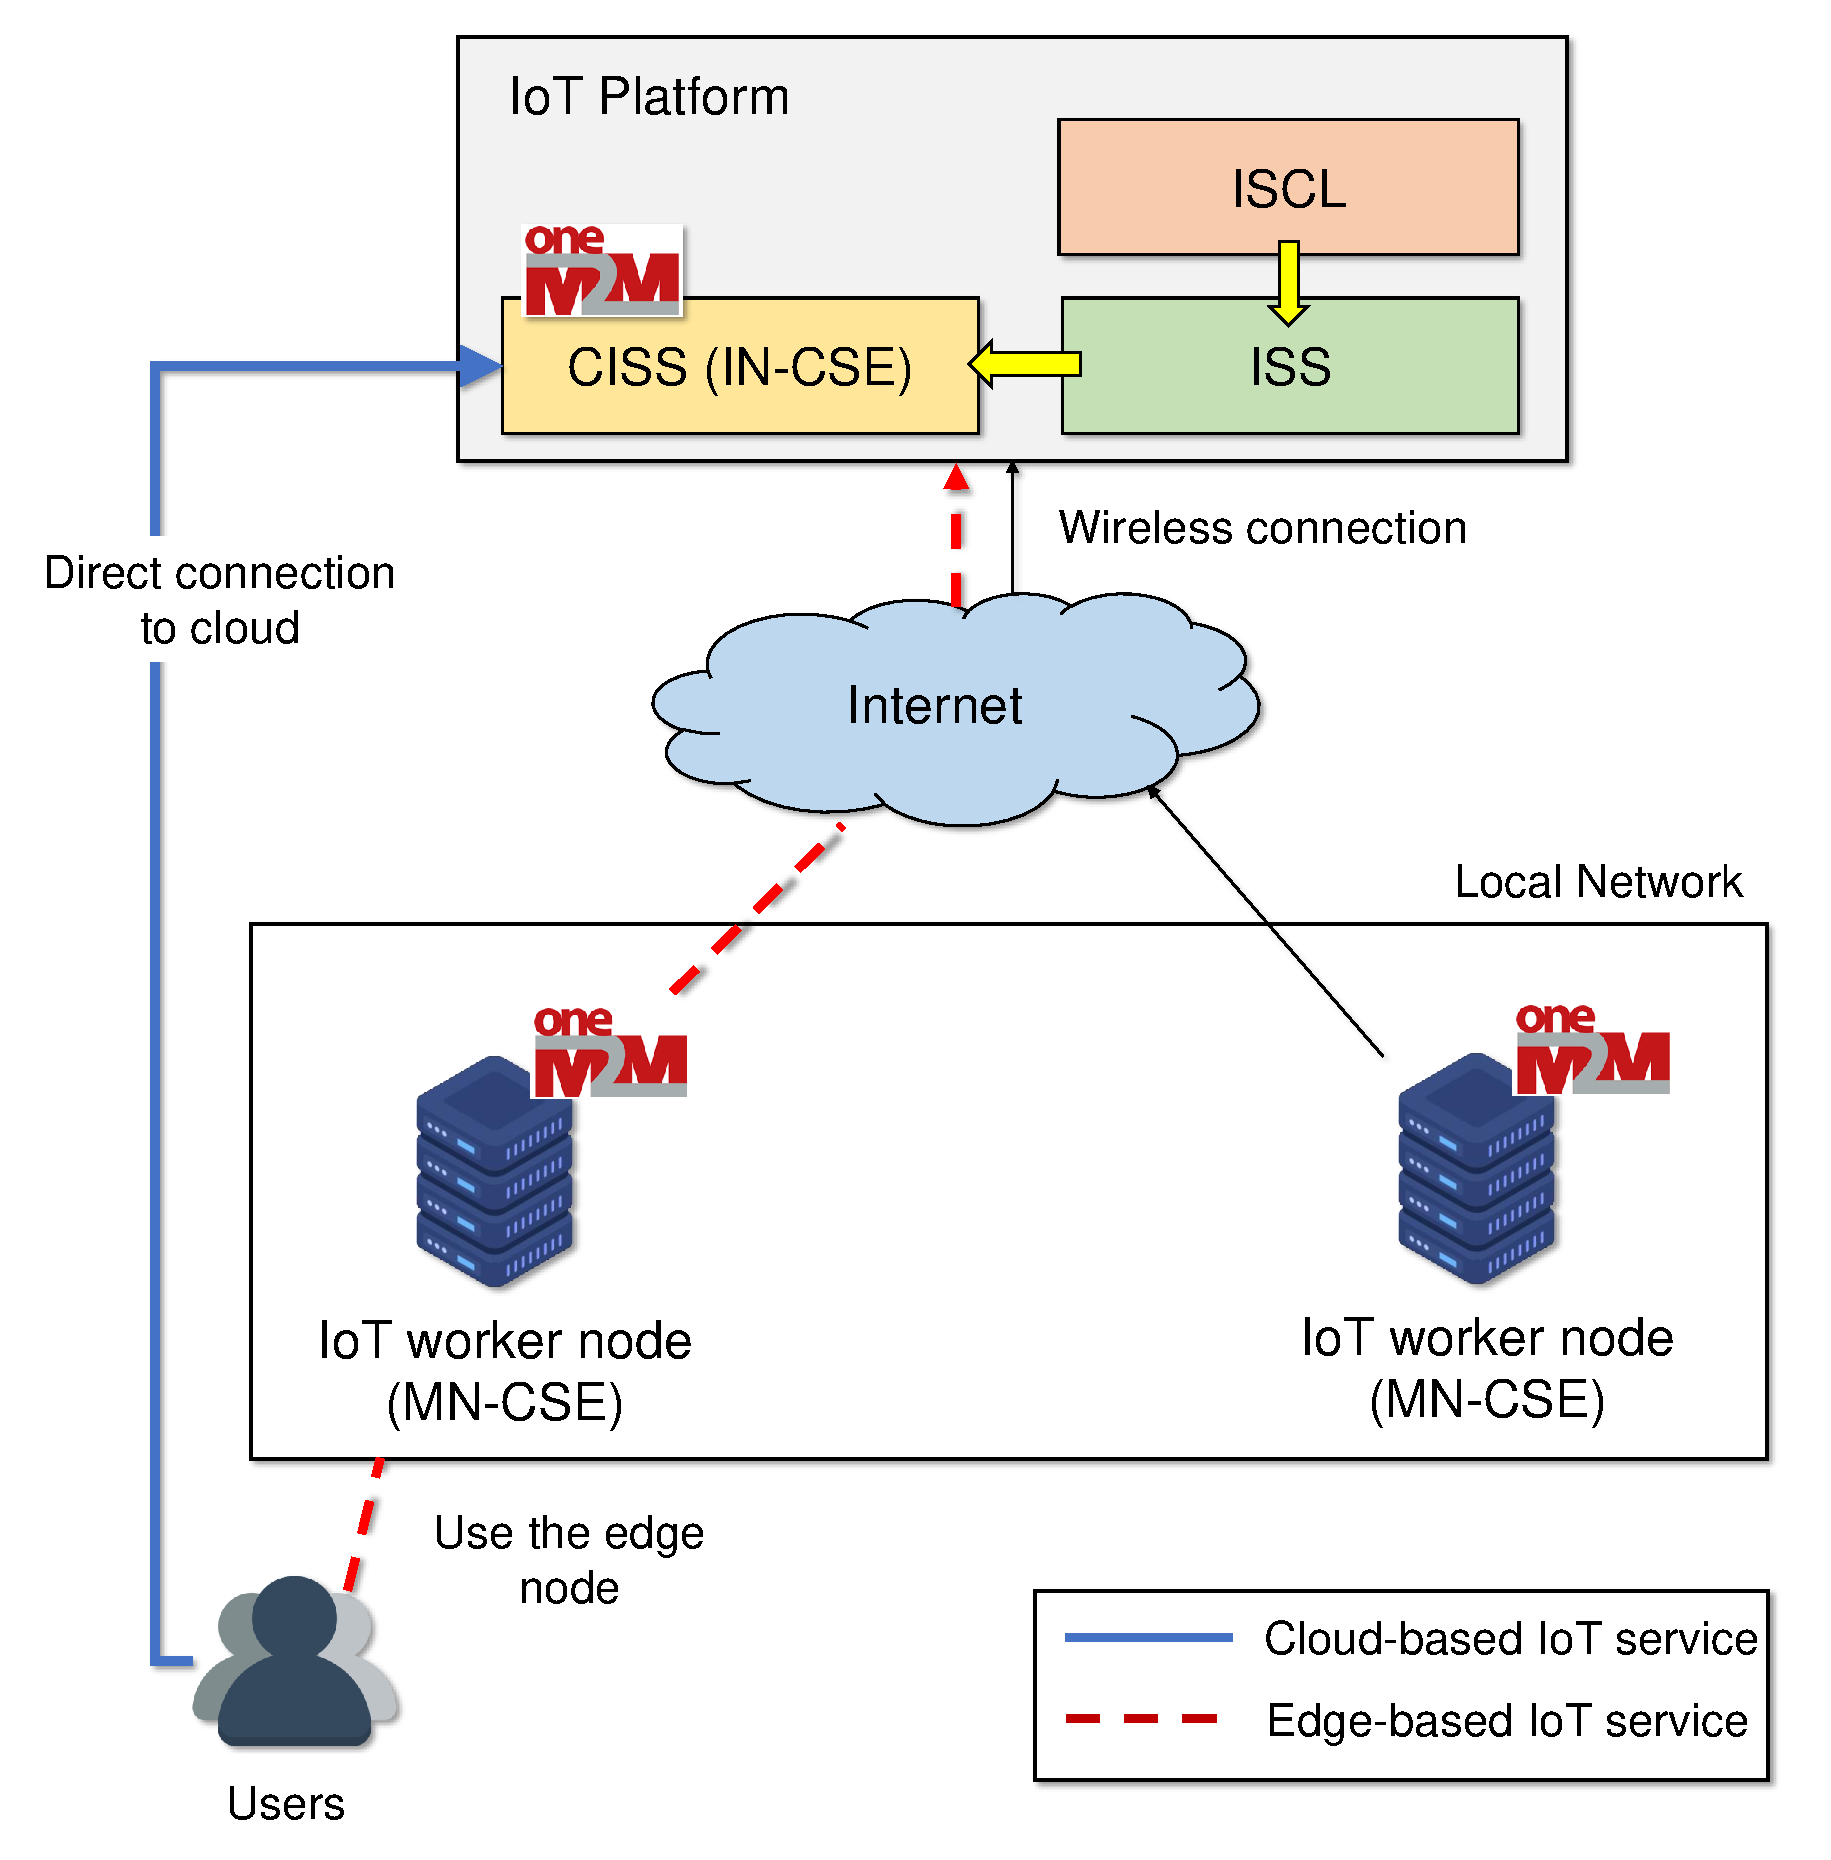
\includegraphics[width=1\columnwidth]
{figures/fig_IoT_slicing_evaluation.pdf}
\caption{IoT service slicing evaluation environment}
\label{fig:iot_service_slicing_environment}
\end{figure}

\begin{figure}[tb!]
\centering
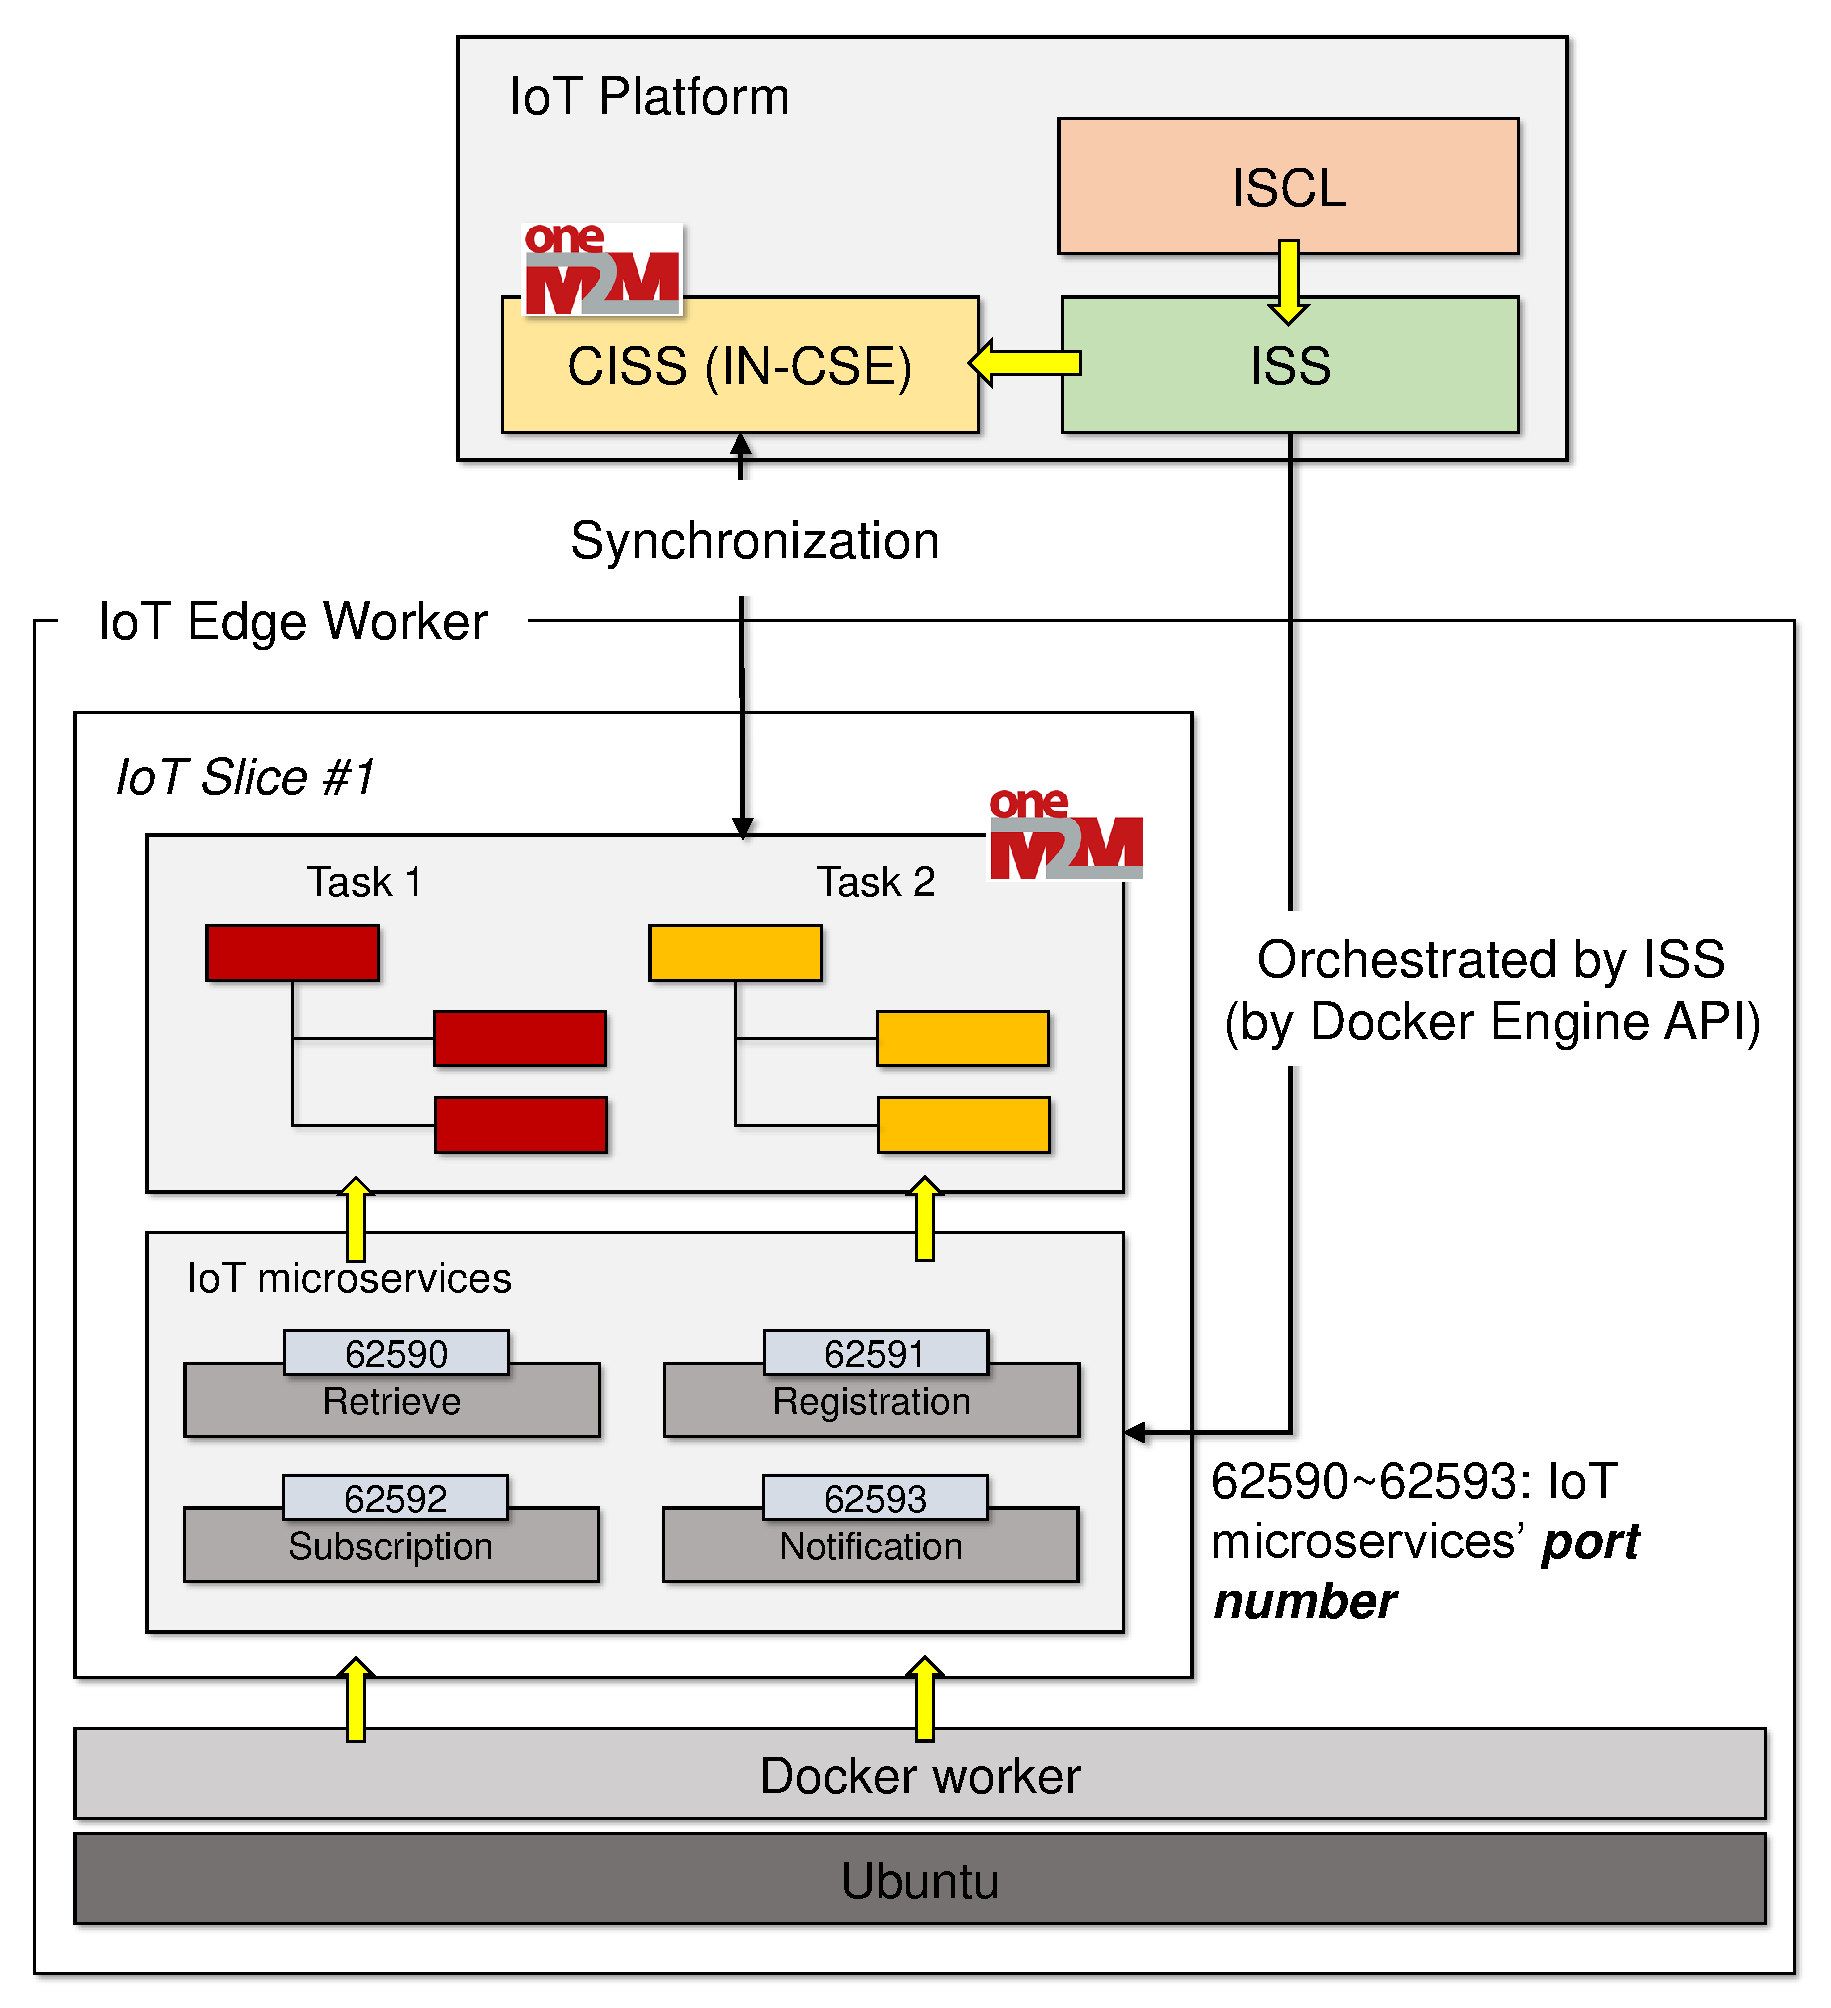
\includegraphics[width=1\columnwidth]
{figures/fig_IoT_slicing_evaluation_docker.pdf}
\caption{IoT service slicing microservices on an edge node}
\label{fig:iot_service_slicing_environment_edge_detail}
\end{figure}

\subsubsection{Evaluation}
%The RTT of both the edge node and cloud is measured by using Apache JMeter. 
The RTT of both scenarios, a cloud-based IoT service and  edge-based IoT service, is measured by using Apache JMeter. 
Apache JMeter is open-source software that tests functional behavior and measures performance. 
This software was first designed to test the web application, but through the extension of the test function, it can test the database and query, FTP server and so on~\cite{jing2010jmeter}. 
As an evaluation method, three performance matrices are used when IoT service slicing and task offloading are finally performed: data update time through the creation of \texttt{<contentInstance>} resource and data retrieval time through the access of \texttt{<contentInstance>} resource. 
In addition, the average performance was presented by measuring the time from requesting to use the edge service to receiving the final completion response.

The data generated in the cloud and the edge node were assumed to continuously change the location of the device so that IoT devices will continually send the changed location as a form of \texttt{<contentInstance>} resources. The size of the \texttt{<contentInstance>} resource used in this comparison is approximately 400 bytes, and in order to measure the performance of \texttt{<contentInstance>} resource creation of both cloud and edge nodes, a request for creation is delivered 60 times, and the result is shown in Fig.~\ref{fig:iot_service_slicing_comparison_generation}. 
When data were delivered to the cloud, the performance distribution of the cloud was averaged at 8.5 ms. 
In addition, when the edge node takes the registration request from the IoT devices, on average, the performance distribution is approximately 6.1 ms. Therefore, in this context, approximately 2.0 ms of performance improvement is expected when edge nodes are brought in.

In addition, checking the data gathering time is one of the important parts of performance evaluation, allowing both the time regarding data generation to be measured and the IoT service-related data to be quickly used. 
Therefore, the most recently generated \texttt{<contentInstance>} resource including location information is used to evaluate the impact of the edge node. At first, the cloud used approximately 67.42 ms on average to respond to the clients. 
In contrast, the edge node spends the time delivering the response at approximately 37.32 ms on average. In summary, by using the edge node, it is likely that users can obtain more seamless IoT services.

\begin{figure}[tb!]
\centering
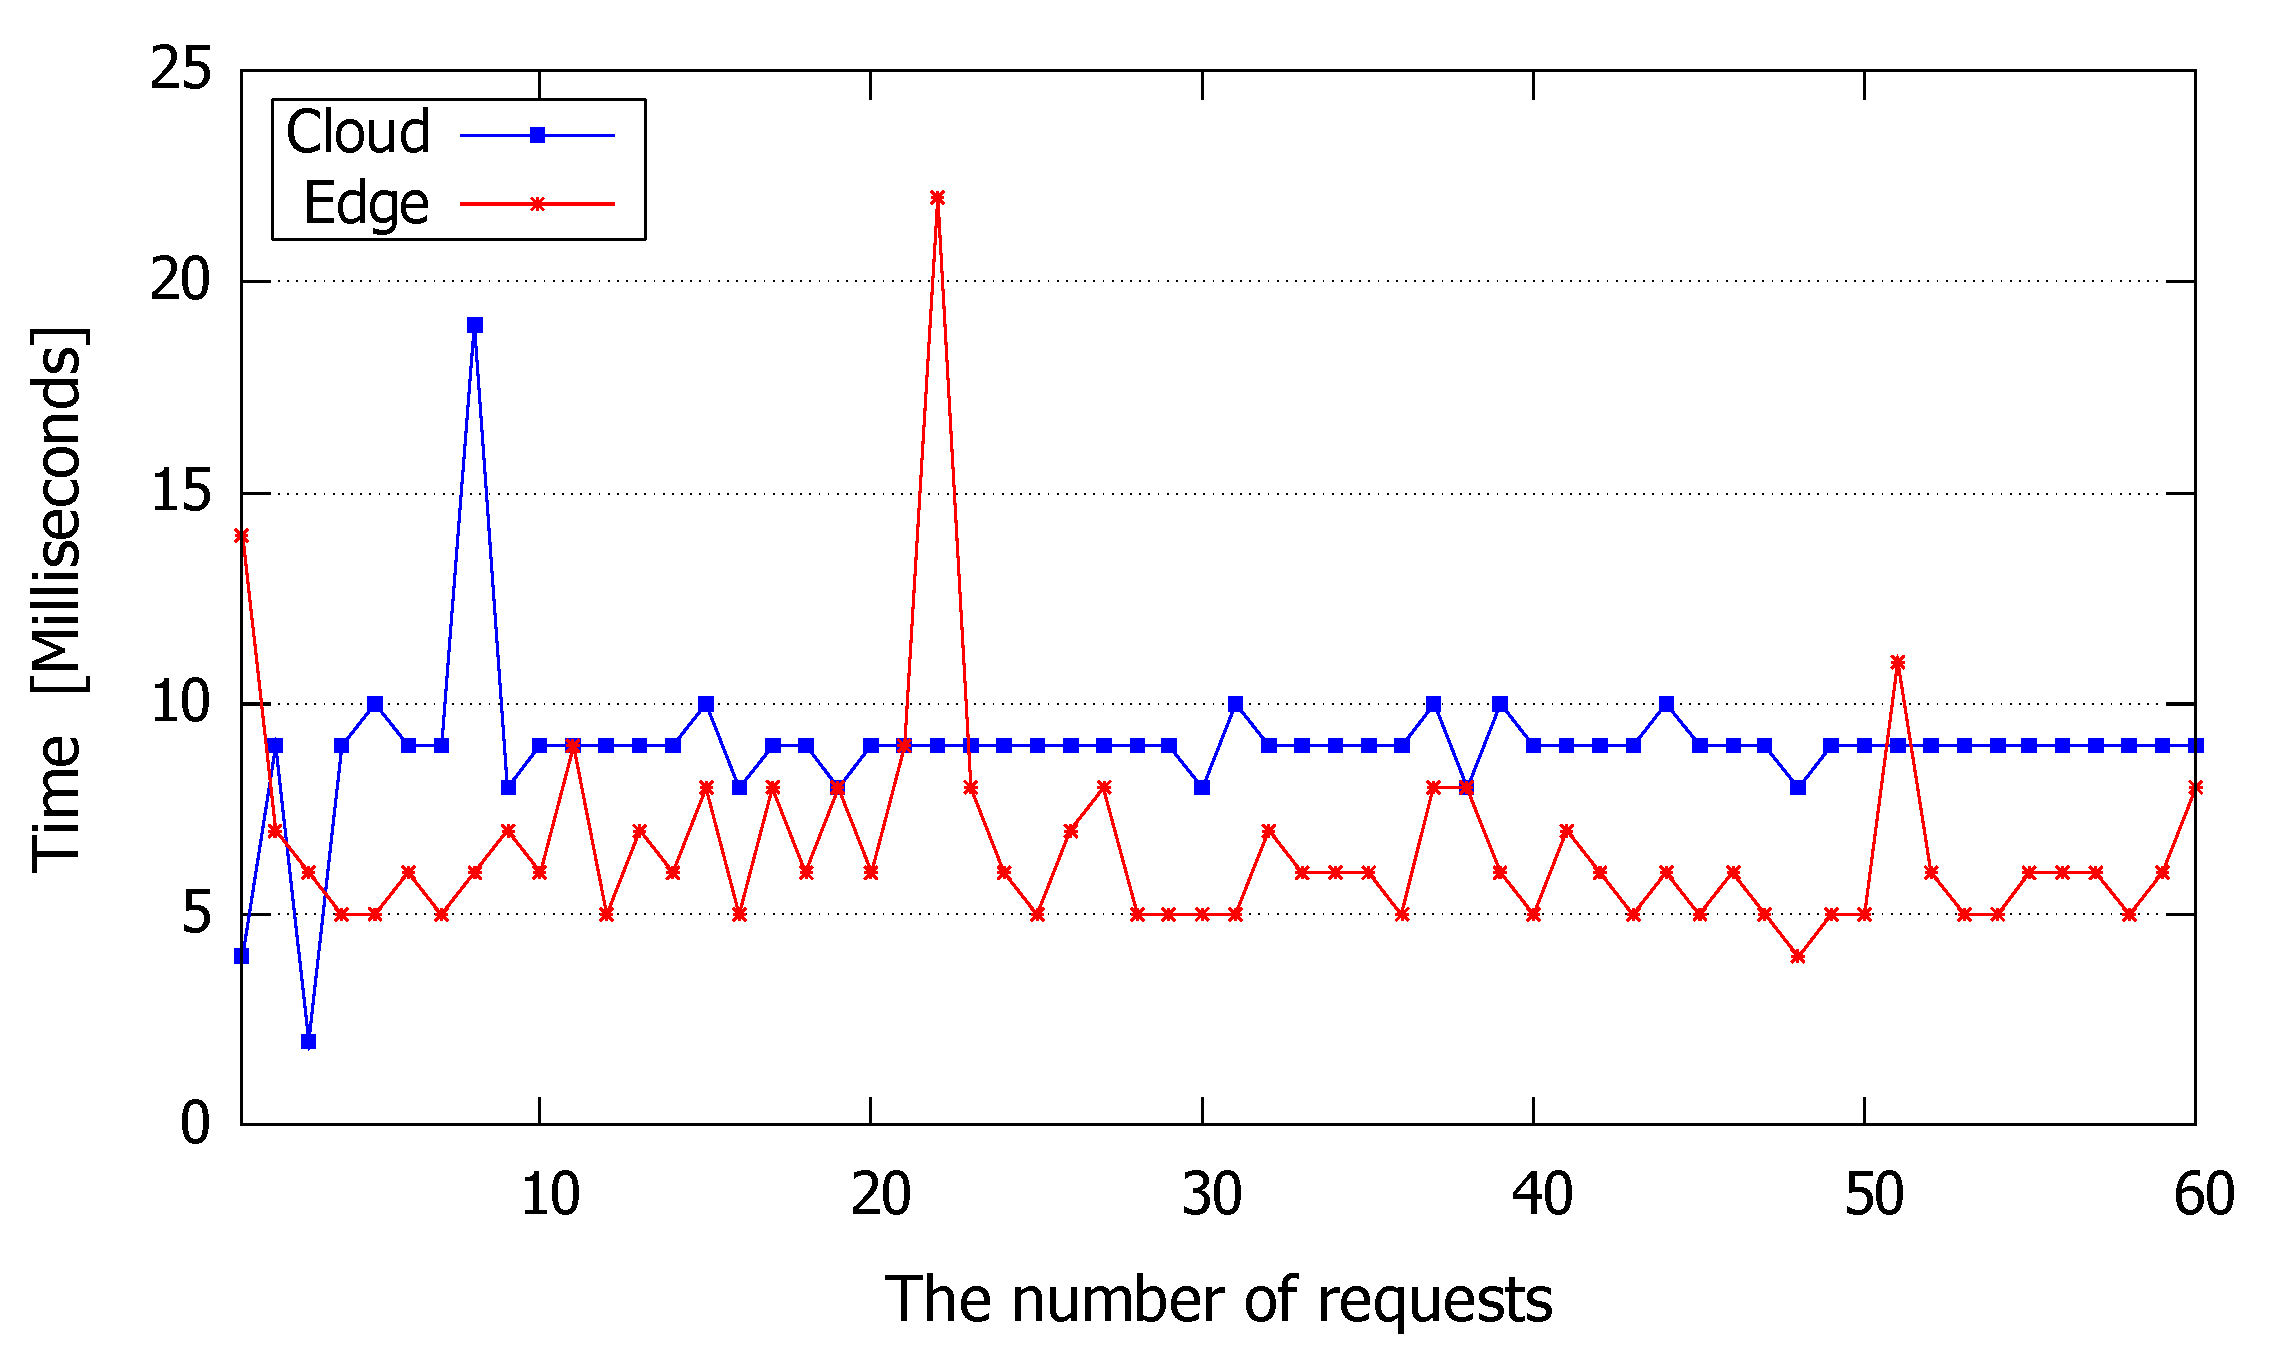
\includegraphics[width=1\columnwidth]
{figures/fig_evaluation_result_creation.pdf}
\caption{Data generation time comparison between cloud and edge modes}
\label{fig:iot_service_slicing_comparison_generation}
\end{figure}

\begin{figure}[tb!]
\centering
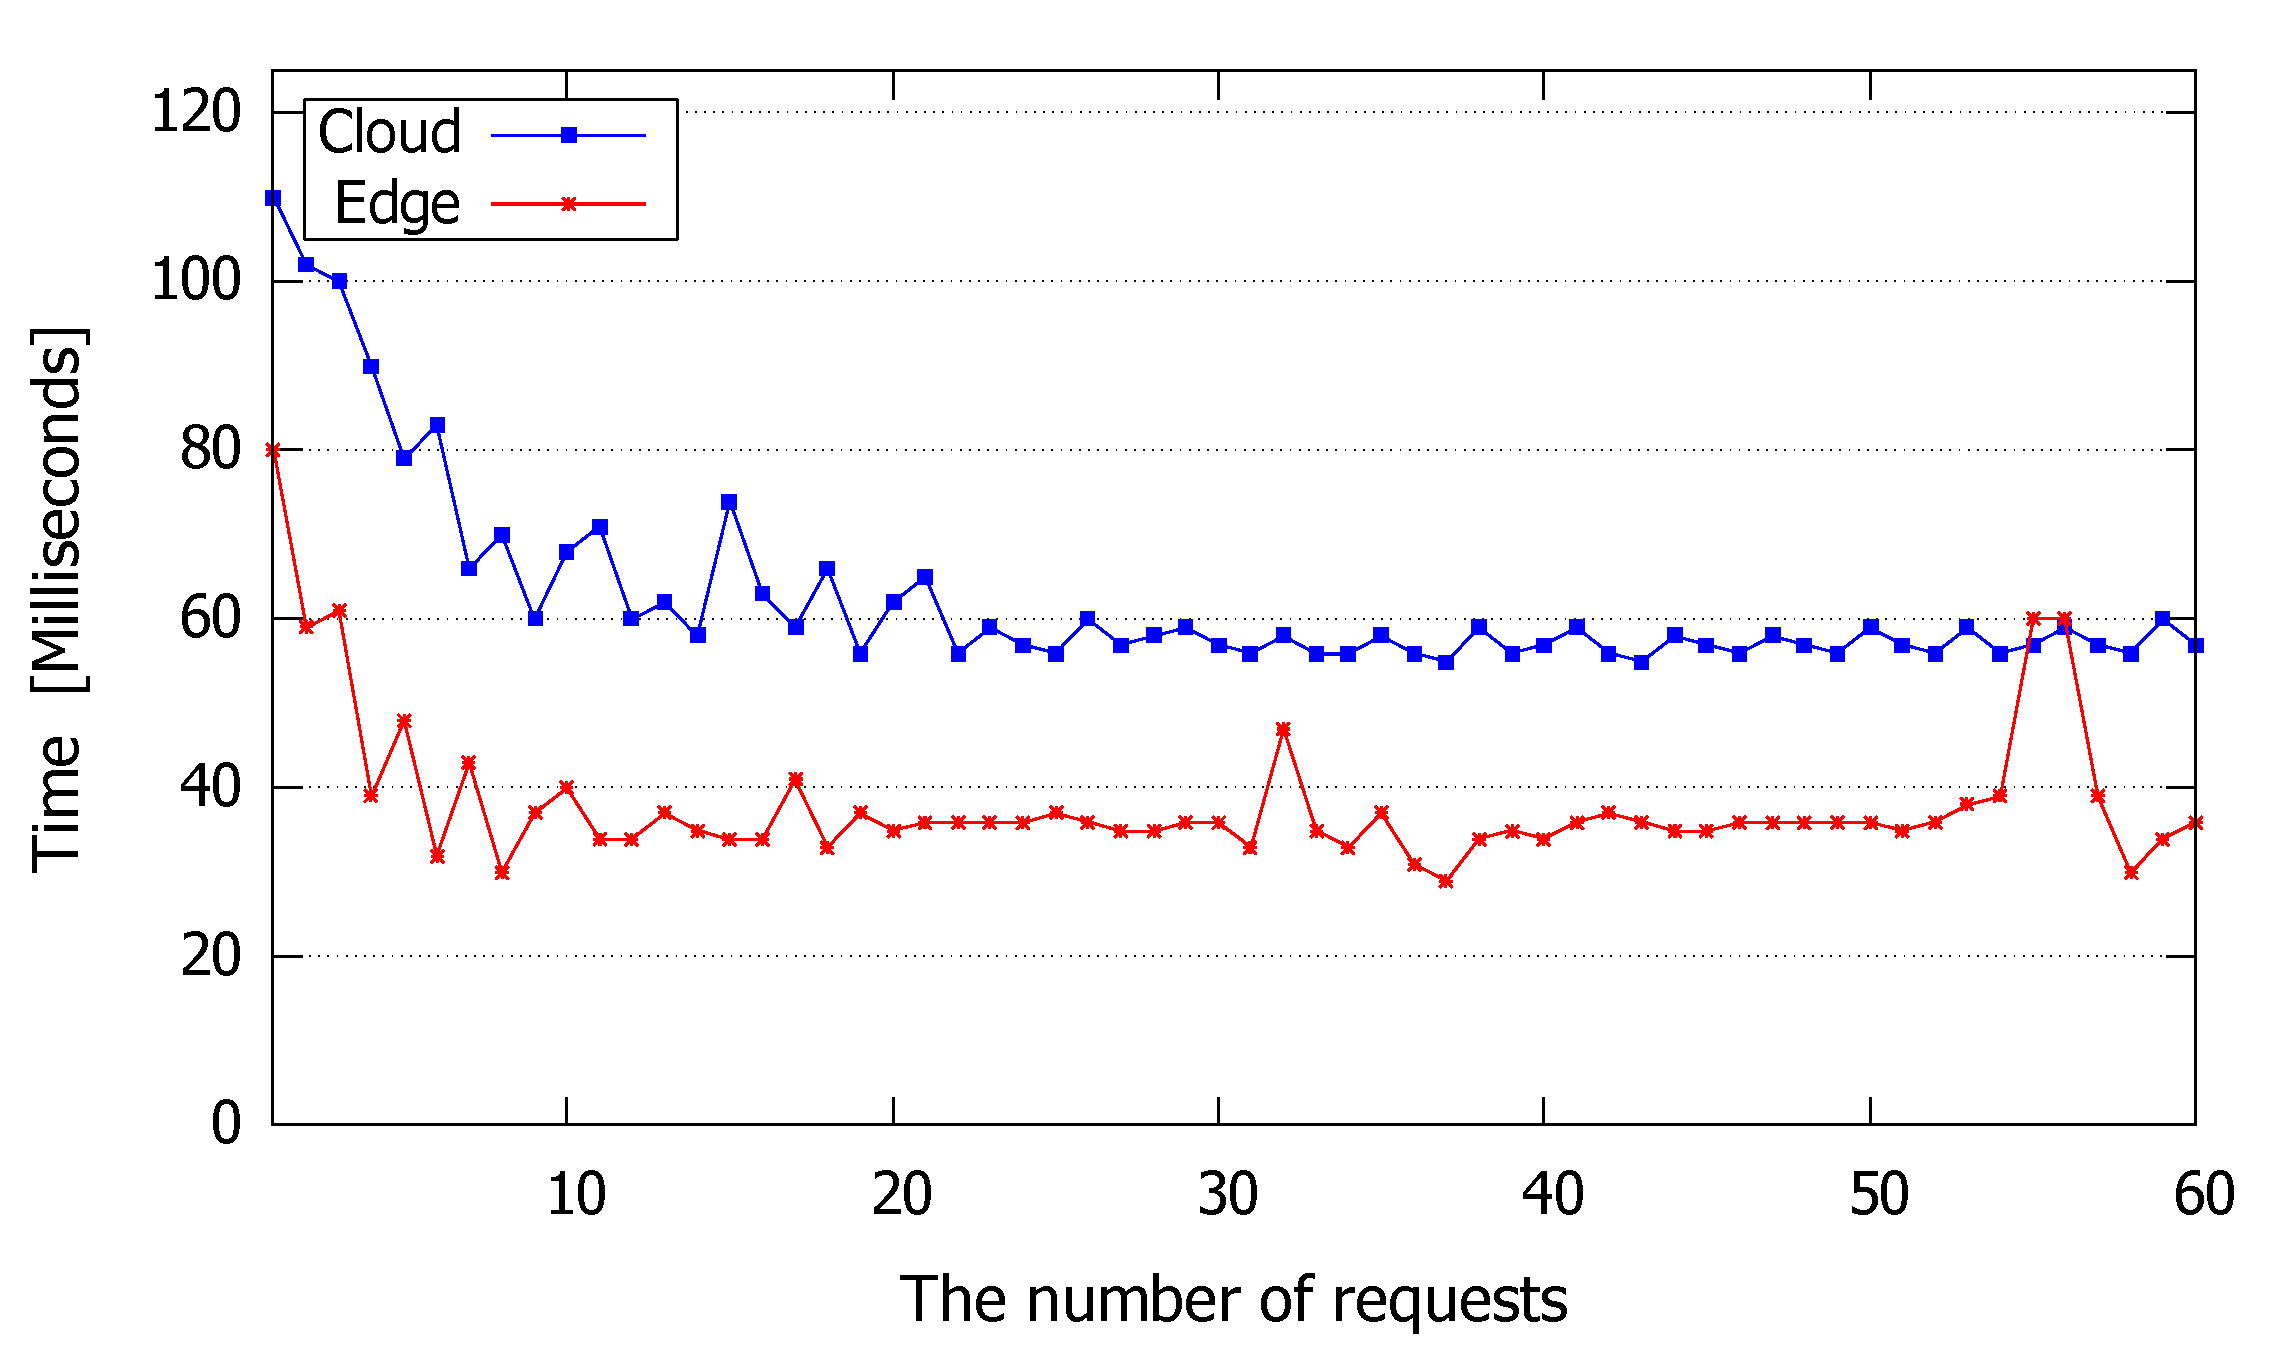
\includegraphics[width=1\columnwidth]
{figures/fig_evaluation_result_retrieve.pdf}
\caption{Data retrieval time comparison between cloud and edge modes}
\label{fig:iot_service_slicing_comparison_retrieve}
\end{figure}

\begin{figure}[tb!]
\centering
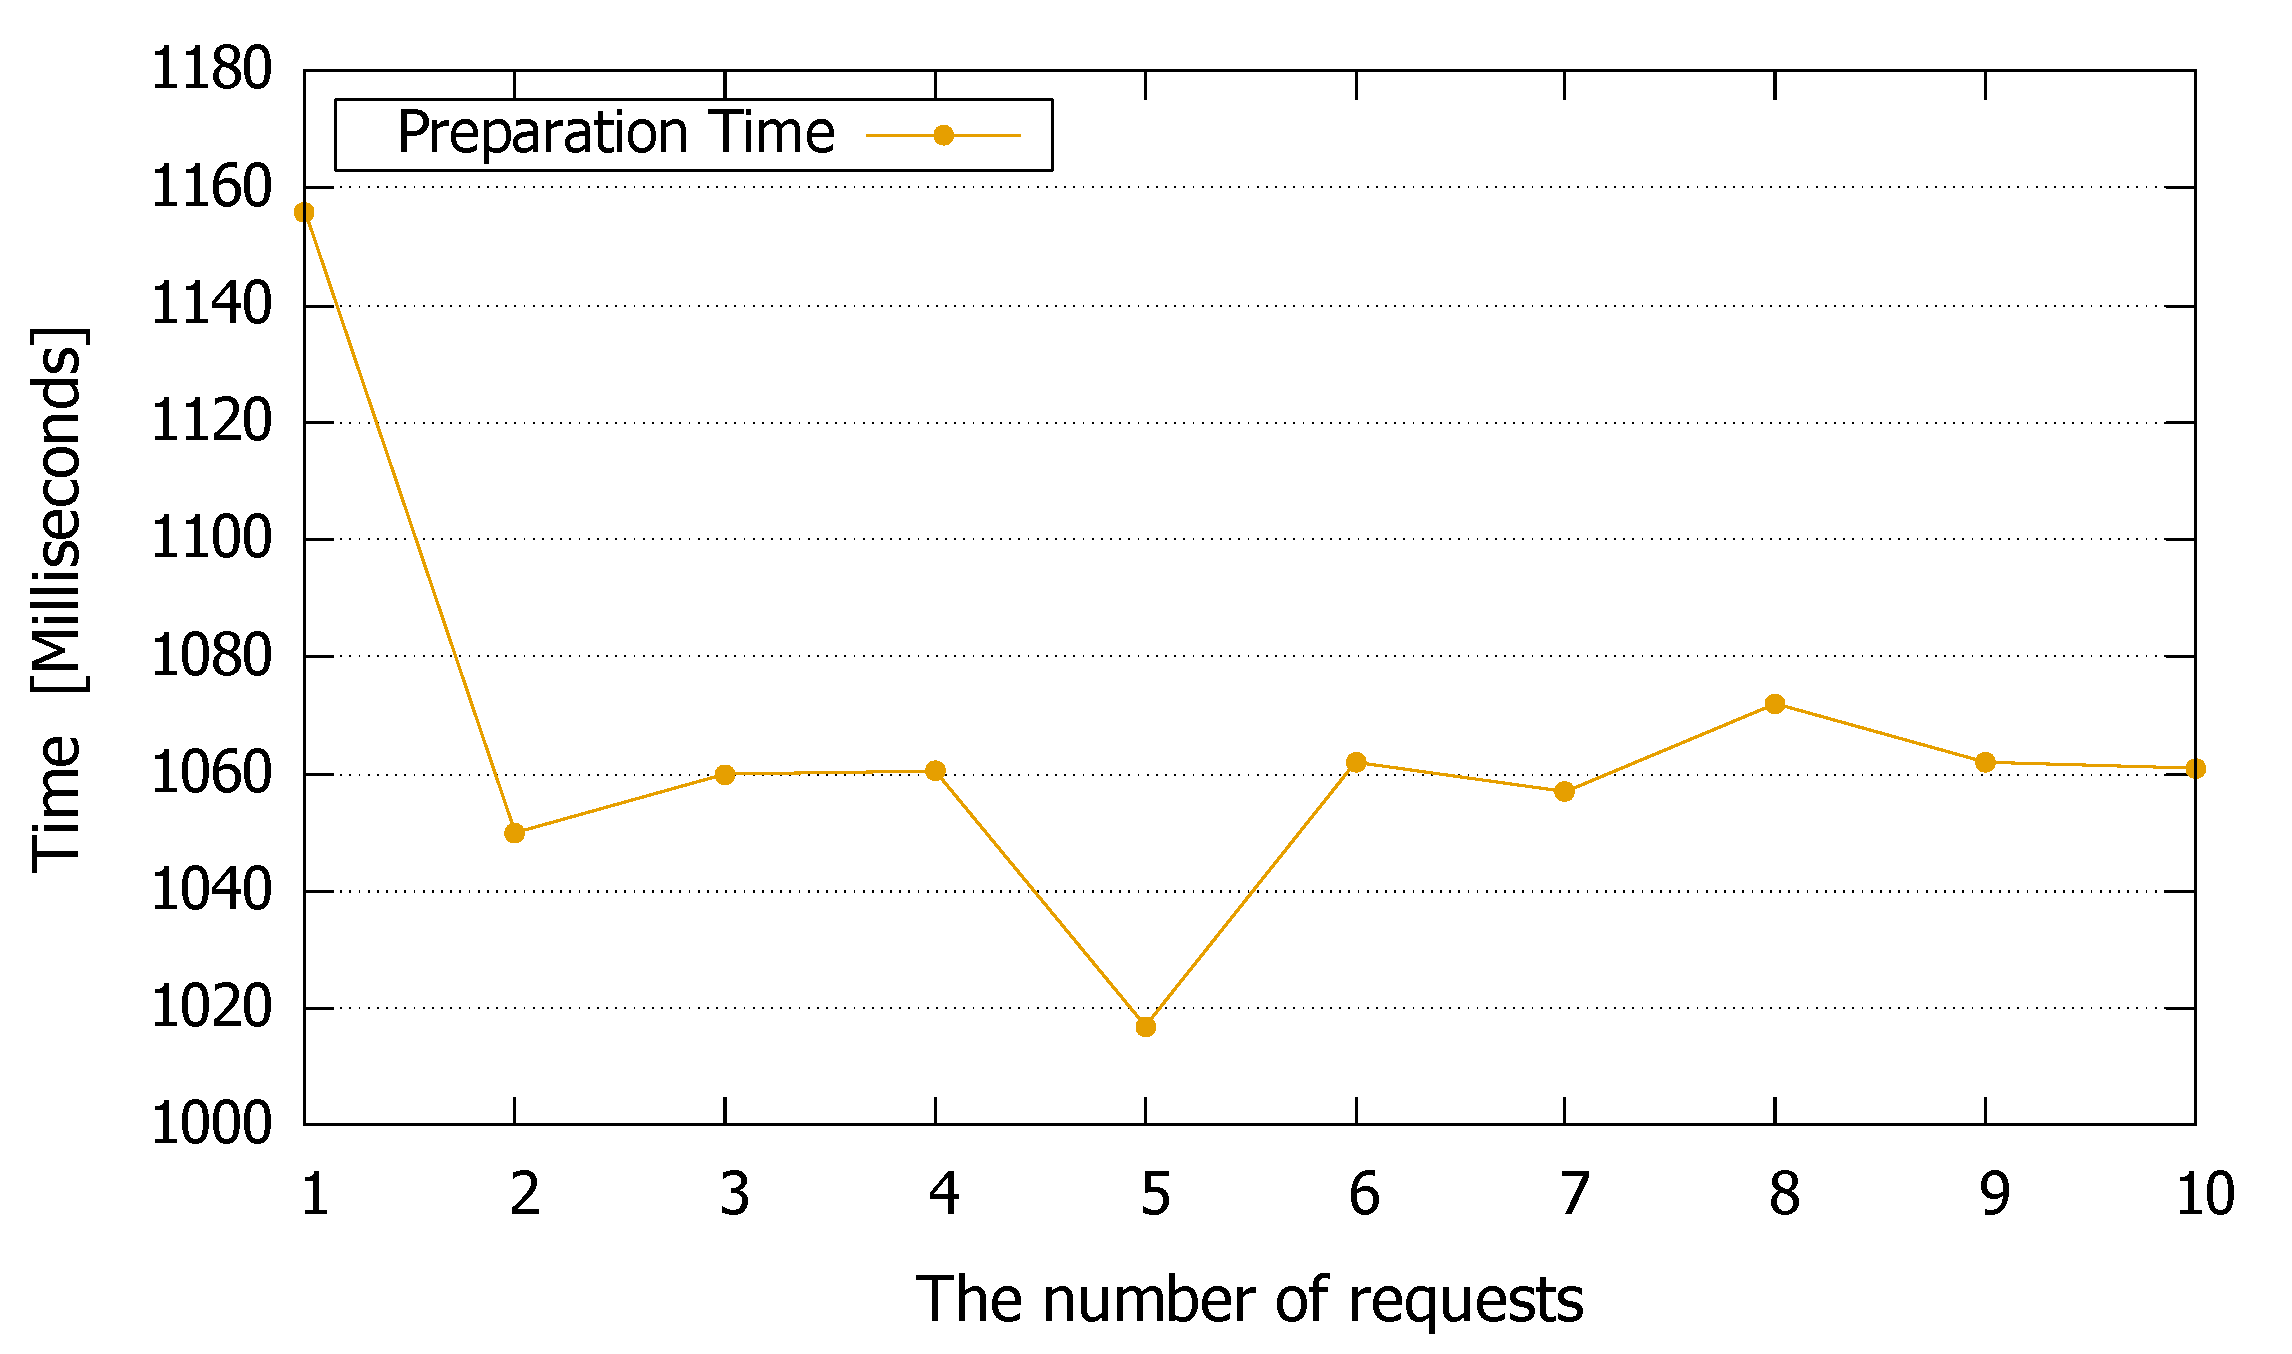
\includegraphics[width=1\columnwidth]
{figures/fig_evaluation_result_preparation.pdf}
\caption{IoT service slicing and IoT task offloading preparation time}
\label{fig:iot_service_slicing_preparation}
\end{figure}

By measuring the IoT service slicing and IoT task offloading time, it is possible to measure the service preparation time for the user to receive the edge node-based IoT services. 
To measure the corresponding time, a total of 10 measurements were performed. As shown in the graph in Figure.~\ref{fig:iot_service_slicing_preparation}, the time of 1.047 ms was measured on average. 
This is the time when the image is already included in the edge node to operate the Docker service. 
If the Docker images are not already placed in the edge node, to download the image, the edge node needs to download the image from the Docker hub, and it might take a long time. 
For example, the size of the Node.js web framework image used in this evaluation is approximately 400 megabytes (MB), and the Python web framework such as Django is approximately 150 MB. 
Therefore, the IoT microservices required for supporting each IoT service do not change significantly unless a function update is required, such as adding a new function, so it may be better to store IoT function images in advance.

\subsection{Summary}
A novel reference architecture for integrating edge computing and IoT platform is proposed. The reference architecture has defined the two core concepts for providing users with IoT services in short distances. IoT service slicing is to constitute the IoT services by selecting the functions required by specific IoT services, and IoT task offloading has been defined for delivering the IoT services operating in the cloud-based IoT platform to the edge nodes. Accordingly, it is expected that the IoT platform can provide the time-sensitive IoT services to the users, which enable IoT service providers can support a variety of new services. In addition, to prove the feasibility of reference architecture, a transmission time performance comparison of edge node-based IoT services and cloud-based IoT services is described. In conclusion, applying the proposed architecture to the edge node and the IoT platform can bring better performance than the existing central-based IoT platforms.
\clearpage